\documentclass[aps,showpacs,twocolumn,twoside,groupedaddress]{revtex4}
\usepackage{graphicx}
\usepackage{epsfig}
%\usepackage{caption}
%\usepackage{subcaption}
\usepackage{epsf}
\usepackage{amssymb}
\usepackage{epstopdf}
\usepackage{amsmath}
\usepackage{braket}
\usepackage{multirow}
\usepackage{array}
\usepackage{mathrsfs}
\usepackage{bm}
\usepackage{wasysym}
\let\vec\bm

\makeatletter
\renewcommand{\fnum@figure}{Fig. \thefigure}
\makeatother

\begin{document}

\title{The steady state population inversion of multiple $\Xi$-type atoms by the squeezed vacuum in a waveguide}
\author{Jieyu You$^{1}$, Zeyang Liao$^{1,2}$, and M. Suhail Zubairy$^{1}$}
\affiliation{$^{1}$Institute for Quantum Science and Engineering (IQSE) and Department of Physics and Astronomy, Texas A$\&$M University, College Station, TX 77843-4242, USA \\
$^{2}$ School of Physics, Sun Yat-sen University, Guangzhou, 510275, China}

\begin{abstract}
We study the dynamics of multiple $\Xi$-type atoms driven by a squeezed vacuum reservoir in a quasi-one-dimensional waveguide. We show that the atomic system's steady state is a pure state, and a complete population inversion can occur when the dipole moment of the second transition is almost perpendicular to the polarization of the incident squeezed light. We also prove that steady state of the system is the direct product of that in the single-atom case even when dipole-dipole interaction is involved. This steady state population inversion may be used to study the two-photon laser or collective atomic effect.
\end{abstract}
\pacs{42.30.-d, 42.50.Hz, 42.62.Fi}\maketitle 


\section{Introduction}
The concept of population inversion is of fundamental importance in laser physics because the production of population inversion is a key step in the workings of a standard laser. However, a population inversion can never exist for a system at thermal equilibrium because of the spontaneous emission. The achievement of population inversion therefore requires pushing the system into a non-equilibrated state \cite{svelto1998principles}. Thus, the spontaneous emission must be inhibited in order to maintain the population inversion in a steady state. In 1946, Purcell showed that the spontaneous decay rate of an emitter can be modified by engineering the electromagnetic bath environment with which the emitters interact \cite{purcell1946purcell}. One famous example of bath engineering is the squeezed vacuum which leads to many novel effects and techniques in quantum optics and atomic spectroscopy. The reduction of quantum fluctuations below vacuum level by the squeezed vacuum yields many interesting phenomenons, for example, the suppression of dephasing rate in one direction and enhancment in the other for a two-level emitter \cite{gardiner1986cw, collett1984mj,gea1988vacuum,palma1989gm, agarwal1990cooperative, ficek1990spontaneous,ficek1991z, goldstein1996ev}, the subnatural linewidth of resonance fluorescence \cite{carmichael1987, toyli2016resonance}, and improvement of an atomic clock using squeezed vacuum\cite{Kruse}. The entanglement nature of the squeezed vacuum also leads to interesting results like pairwise excitation of atomic states \cite{tanas2004stationary, li2006preparing, You2018}. In 1993, Ficek et. al. studied the dynamical properties of a three-level atom in the squeezed vacuum where they showed that a three-level atom in the cascade configuration coupled to squeezed modes can reach steady state level populations inversion relative to ordinary laser spectroscopy \cite{ficek1991three, ficek1993two}. 

Recently, photon transport in a one-dimensional (1D) waveguide coupled to quantum emitters (well known as "waveguide-QED") has attracted much attention because it can not only enhance the interaction but also transport information by guiding the photon \cite{shen2005coherent, shen2007strongly, yudson2008multiphoton, liao2015single, liao2016dynamical, liao2016review, roy2017review}. However, in these studies, the photon modes are usually considered to be ordinary vacuum modes. Although the squeezing of all modes in three dimensions is difficult, the squeezing of modes in one dimension is experimentally feasible.  Suppression of the radiative decay of atomic coherence and the linewidth of the resonance fluorescence have been experimentally demonstrated in a 1D microwave transmission line coupled to single artificial atom \cite{turchette1998qa, murch2013kw, toyli2016resonance, bergeal2010analog, wang2018cavity, qin2018exponentially}.  %Since squeezing in 1D is more experimentally feasible than squeezing all modes in 3D space, in our study, we are considering multiple $\Xi$-type atoms coupled to the broadband squeezed vacuum in the quasi-one-dimensional waveguide. We show that for a single atom, the steady state is the superposition of the ground state and the second excited state and the population inversion can approach $100\%$. This result is similar to the result in the cavity case shown in Ref. \cite{ficek1991three}. Furthermore we also mathematically prove that this result can be generalized to arbitrary amount of atoms coupled to each other through dipole-dipole interaction, which may be a scenario for studying the subradiance effect.

%The paper is organized as follows. In Sec. II, we derive the master equation for multiple three-level atoms coupled to the squeezed vacuum in a 1D waveguide. In Sec. III, we derive the steady state of a single three-level atom driven by squeezed vacuum in 1D waveguide and compare it to the result in Ref. \cite{ficek1991three}. In Sec. IV, we consider the case with multiple atoms which can have dipole-dipole interactions. Finally, we summarize the result.


Thus, Ref. \cite{ficek1991three, ficek1993two}'s proposal on the steady state popoulation inversion seems to be experimentally implementable by coupling an atom with one dimensional squeezed modes. However, there are still three issues in their proposal: first, the steady state population distribution cannot be controlled because the atomic decay rate is not tunable; second, only a single independent atom is considered to be interacting with the squeezed vacuum, while the dipole-dipole interaction between atoms may affect the steady state population distribution; third, the effect of squeezing source is not included as discussed in Ref.\cite{You2018}. Our goal is to fix these issues.  

In our study, we consider multiple $\Xi$-type atoms coupled to the broadband squeezed vacuum in the quasi-one-dimensional waveguide where all resonant modes can be technically squeezed. We show that for a single atom, it can always reach a population inversion of almost $100\%$ or any other ratio as long as the direction of its transition dipole moment is properly set. We also mathematically prove that this result can be generalized to arbitrary amount of atoms coupled to each other through dipole-dipole interaction, which may be a scenario for studying two-photon laser or collective atomic effect.

\section{Master equation of three-level atoms in the squeezed vacuum}

In this section, we consider a scenario where $N_a$ $\Xi$-type atoms are located inside a perfect rectangular waveguide with the squeezed vacuum injected from both ends, as shown in Fig.~\ref{1}(a). The atomic electronic structure is shown in Fig.~\ref{1}(b) where the atomic states are labeled as $|a\rangle$, $|b\rangle$, $|c\rangle$ from the excited state to the ground state. Different from the free space, the square waveguide can only support certain photon modes, i.e., $TE_{mn}$ and $TM_{mn}$ modes with cutoff frequency $c\sqrt{(\frac{m\pi}{a})^{2}+(\frac{n\pi}{b})^{2}}$, where $a \times b$ is the dimension of the waveguide's cross section. For the rectangular waveguide, there is no $TM_{01}$ or $TM_{10}$ mode. Assuming $b<a$, $TE_{10}$ is the ground mode with the lowest cutoff frequency. Thus, the atom is only coupled to $TE_{10}$ mode as long as $\frac{\pi c}{a}<\omega_{ab},\omega_{bc}<min(\frac{\pi c}{b},\frac{2\pi c}{a})$. We assume that $\omega_{ac}=2\omega_0$ where $\omega_0$ is the center frequency of the broadband squeezed vacuum. We also assume that the squeezed vacuum bandwidth is much larger than $|\omega_{ab}-\omega_{bc}|$ so it forms a squeezed vacuum reservoir. 
\begin{figure*}
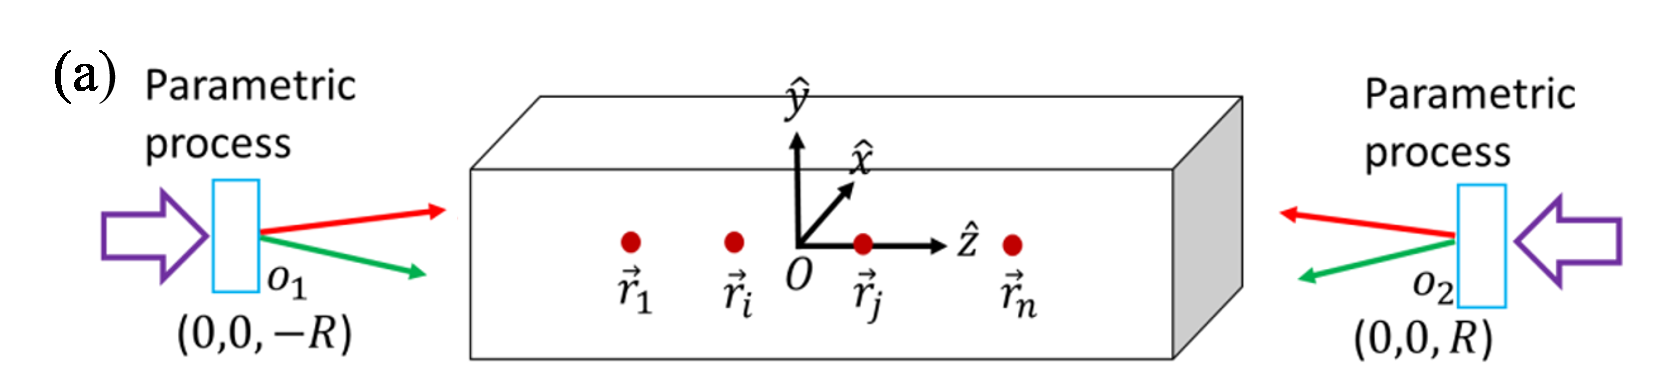
\includegraphics[width=1.5\columnwidth]{fig1.eps}
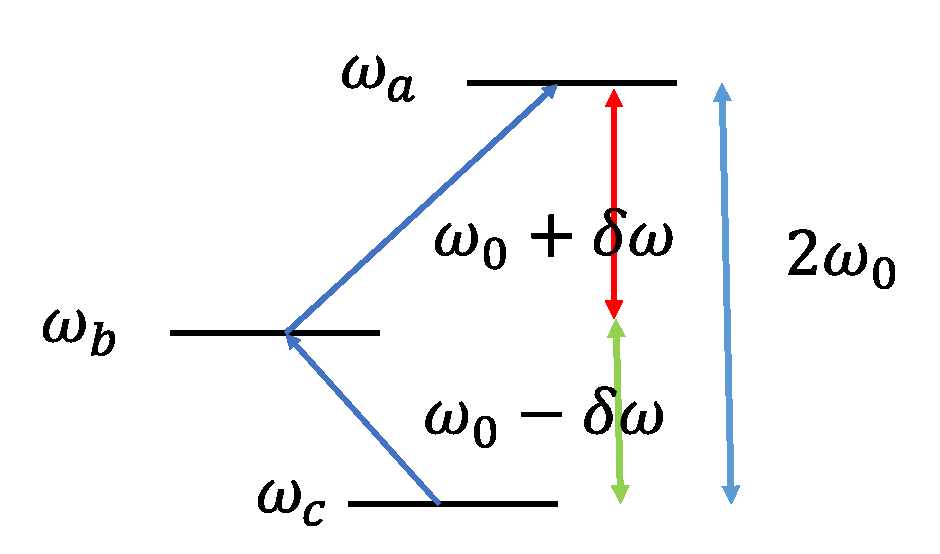
\includegraphics[width=0.5\columnwidth]{fig2.eps}
\caption{(a) Schematic setup: A $\Xi$-type atom is located inside the waveguide with the broadband squeezed vacuum incident from both ends. (b)The energy structure of the three level atom. Transition $|a\rangle\rightarrow|c\rangle$ is forbidden and $\omega_{ac}=2\omega_0$ where $\omega_0$ is the center frequency of the squeezed vacuum. $\omega_{ab}$ and $\omega_{bc}$ differ by a small amount $2\delta\omega_0$ and they are within the bandwidth of the squeezed vacuum reservoir.}
\label{1}
\end{figure*}


%The general master equation of dipole-dipole interaction in the squeezed vacuum can be used to study the dynamics of the three-level atom\cite{You2018}:

The atom-field system is described by the Hamiltonian \begin{equation}
  \label{hamltonian}
  \begin{gathered}
H=H_{A}+H_{F}+H_{AF}
 \end{gathered}
\end{equation}
where
$H_{A}=\sum_{l=1}^{N_a}\sum_{e=a,b,c}\hbar\omega_{e,l}\left|e_{l}\right\rangle \left\langle e_{l}\right|$  
is the atomic Hamiltonian, and $ \left|e_{l}\right\rangle $ is the energy state of the $l$th atom with energy $\hbar\omega_{e,l}$. The Hamiltonian of the EM field is
$H_{F}=\sum_{\vec{k}s}\hbar\omega_{\vec{k}s}(\hat{a}_{\vec{k}s}^{\dagger}\hat{a}_{\vec{k}s}+\frac{1}{2})$
where $\hat{a}_{\vec{k}s}$ and $\hat{a}_{\vec{k}s}^{\dagger}$ are the annihilation and creation operators of the filed mode with wavevector $ \vec{k}$, polarization $s$ (in waveguide, it represents $TE_{mn}$ or $TM_{mn}$), and frequency $\omega_{\vec{k},s}$. The interaction Hamiltonian in electric-dipole approximation is
$H_{AF}=-i\hbar\sum_{\vec{k}s}\sum_{i=1,2}\sum_{l=1}^{N_{a}}[\vec{\mu}_{l,i}\cdot\vec{u}_{\vec{k}s}(\vec{r}_{l,i})S_{l,i}^{+}\hat{a}_{\vec{k}s}+\vec{\mu}_{l,i}^{*}\cdot\vec{u}_{\vec{k}s}(\vec{r}_{l,i})S_{l,i}^{-}\hat{a}_{\vec{k}s}-H.c.]$
where $ \vec{\mu}_{l,i} $ is the electric dipole moment for $ith$ transition of the $l$th atom, where $i=1$ denotes the transition from $|a\rangle$ to $|b\rangle$, and $i=2$ denotes the transition from $|b\rangle$ to $|c\rangle$. $ S_{l,i}^{+} $ and $S_{l,i}^{-} $ are the raising and lowering operator for transition $i$ of the $l$th atom. The mode function of the squeezed vacuum in $TE_{10}$ mode is given by
\begin{equation}
  \label{eq2b}
  \begin{gathered}
\vec{u}_{\vec{k}s}(\vec{r}_{i})=\sqrt{\frac{\omega_{\vec{k}s}}{2\epsilon_{0}\hbar V}}\vec{x}e^{i\vec{k}\cdot(\vec{r}_{i}-\vec{o}_{\vec{k}s})}
 \end{gathered}
\end{equation}
where $\vec{o}_{\vec{k}s} $ is a phenomenological parameter which includes the effects of the initial phase and the position of the squeezing source\cite{You2018}. The correlation functions for the squeezed vacuum are\cite{scully1999quantum}:
\begin{equation}
\label{eq0a}
\begin{split}
& \left\langle a_{\vec{k},s}^{\dagger}a_{\vec{k}',s'}\right\rangle =\sinh^{2}r\delta_{\vec{k}'\vec{k}}\delta_{ss'} \\
& \left\langle a_{\vec{k},s}a_{\vec{k}',s'}^{\dagger}\right\rangle =\cosh^{2}r\delta_{\vec{k}'\vec{k}}\delta_{ss'}\\
& \left\langle a_{\vec{k},s}^{\dagger}a_{\vec{k}',s'}^{\dagger}\right\rangle =-e^{-i\theta}\cosh(r)\sinh(r)\delta_{\vec{k}',2\vec{k}_{0}-\vec{k}}\delta_{ss'}\\
&\left\langle a_{\vec{k},s}a_{\vec{k}',s'}\right\rangle =-e^{i\theta}\cosh(r)\sinh(r)\delta_{\vec{k}',2\vec{k}_{0}-\vec{k}}\delta_{ss'}
\end{split}
\end{equation}
For simplicity, we can set the squeezing parameter $\theta=0$, and the dipole moments of all atoms to align along the same direction. The dynamics of the atomic system can be described by the following master equation (See Appendix A for details of derivation):
\begin{widetext}
\begin{equation}
\label{eq1}
\begin{split}
\frac{d\rho^{S}}{dt}=&-i\underset{ijkl}{\sum}\Lambda_{ijkl}[S_{i,j}^{+}S_{k.l}^{-},\rho^{S}]e^{i(\omega_{j}-\omega_{l})t}-\frac{1}{2}\underset{ijkl}{\sum}\gamma{}_{ijkl}(1+N)(\rho^{S}S_{i,j}^{+}S_{k.l}^{-}+S_{i,j}^{+}S_{k.l}^{-}\rho^{S}-2S_{k.l}^{-}\rho^{S}S_{i,j}^{+})e^{i(\omega_{j}-\omega_{l})t}\\
&-\frac{1}{2}\underset{ijkl}{\sum}\gamma{}_{ijkl}N(\rho^{S}S_{i,j}^{-}S_{k.l}^{+}+S_{i,j}^{-}S_{k,l}^{+}\rho^{S}-2S_{k,l}^{+}\rho^{S}S_{i,j}^{-})e^{-i(\omega_{j}-\omega_{l})t}\\
&-\frac{1}{2}\sum_{\alpha=\pm}\underset{ijkl}{\sum}\gamma'_{ijkl}Me^{2\alpha ik_{0z}R}e^{i\alpha(\omega_{j}+\omega_{l}-2\omega_{0})t}(\rho^{S}S_{i,j}^{\alpha}S_{k.l}^{\alpha}+S_{i,j}^{\alpha}S_{k,l}^{\alpha}\rho^{S}-2S_{k,l}^{\alpha}\rho^{S}S_{i,j}^{\alpha})
\end{split}
\end{equation}
\end{widetext}
where $N=\sinh(r)^2$, $M=\sinh(r)\cosh(r)$, and the coefficients are
\begin{equation}
\label{eq2}
\begin{split}
& \gamma_{ijkl}=\sqrt{\gamma_{j}\gamma_{l}}\cos(k_{0z}r_{ik}) \\
& \Lambda_{ijkl}=\frac{\sqrt{\gamma_{j}\gamma_{l}}}{2}\sin(k_{0z}r_{ik})\\
& \gamma'_{ijkl}=\sqrt{\gamma_{j}\gamma_{l}}\cos[k_{0z}(r_{i}+r_{k})]
\end{split}
\end{equation}
where subscripts $i,k$ label the atom index, $j(l)$ labels the transitions of the $ith (kth)$ atom. $\gamma_{1}(\gamma_{2})$ is the decay rate for transition $|a\rangle\rightarrow|b\rangle(|b\rangle\rightarrow|c\rangle)$ in ordinary vacuum in the waveguide. Contrary to the free space where the decay rate is independent of the dipole direction, the anisotropy characteristics of the waveguide results in the sensitivity of atomic decay rate to its dipole direction. Thus, $\gamma_j=\gamma_{jmax}\cos\theta_j$ where $\gamma_{jmax}$ is the value of $\gamma_{j}$ when the transition dipole is parallel to the polarization of the incident squeezed light, and $\cos\theta_j$ is the angle between them.

\section{Steady state of a single atom}

In this section, we will study the steady state of a single atom in the squeezed vacuum reservior. For a single three level atom, we have $r_i=r_k$, and for simplicity we set $R=r_i=0$. Then the steady state of Eq.\eqref{eq1} can be derived by re-writing it as:
%We will discuss the steady state solution to Eq. \eqref{eq1} in two cases: $\delta\omega\ll\sqrt{\gamma_{1}\gamma_{2}}$ and $\delta\omega\apprge\sqrt{\gamma_{1}\gamma_{2}}$. When $\delta\omega\ll\sqrt{\gamma_{1}\gamma_{2}}$, Eq. \eqref{eq1} can be simplified as:
%\begin{equation}
%\label{eq3a}
%\begin{split}
%\frac{d\rho^{S}}{dt}=&-\frac{1}{2}\underset{ij}{\sum}\gamma_{ij}(1+N)(\rho^{S}S_{i}^{+}S_{j}^{-}+S_{i}^{+}S_{j}^{-}\rho^{S}-2S_{j}^{-}\rho^{S}S_{i}^{+})\\
%&-\frac{1}{2}\underset{ij}{\sum}\gamma_{ij}N(\rho^{S}S_{i}^{-}S_{j}^{+}+S_{i}^{-}S_{j}^{+}\rho^{S}-2S_{j}^{+}\rho^{S}S_{i}^{-})\\
%&-\frac{1}{2}\sum_{\alpha=\pm}\underset{ij}{\sum}\gamma_{ij}'M(\rho^{S}S_{i}^{\alpha}S_{j}^{\alpha}+S_{i}^{\alpha}S_{j}^{\alpha}\rho^{S}-2S_{j}^{\alpha}\rho^{S}S_{i}^{\alpha})
%\end{split}
%\end{equation}

\begin{widetext}
\begin{subequations}
\begin{align}
&\dot{\rho}_{aa}=-\gamma_{1}ch^{2}\rho_{aa}+\gamma_{1}sh{}^{2}\rho_{bb}-\frac{1}{2}\sqrt{\gamma_{1}\gamma_{2}}chsh(e^{-i(\omega_{1}+\omega_{2}-2\omega_{0})t}\rho_{ac}+e^{i(\omega_{1}+\omega_{2}-2\omega_{0})t}\rho_{ca})\label{4a} \\
&\dot{\rho}_{bb}=\gamma_{1}(ch^{2}\rho_{aa}-sh^{2}\rho_{bb})+\gamma_{2}(sh^{2}\rho_{cc}-ch^{2}\rho_{bb})+\sqrt{\gamma_{1}\gamma_{2}}chsh(e^{-i(\omega_{1}+\omega_{2}-2\omega_{0})t}\rho_{ac}+e^{i(\omega_{1}+\omega_{2}-2\omega_{0})t}\rho_{ca})\label{4b}\\
&\dot{\rho}_{cc}=\gamma_{2}ch^{2}\rho_{bb}-\gamma_{2}sh^{2}\rho_{cc}-\frac{1}{2}\sqrt{\gamma_{1}\gamma_{2}}chsh(e^{-i(\omega_{1}+\omega_{2}-2\omega_{0})t}\rho_{ac}+e^{i(\omega_{1}+\omega_{2}-2\omega_{0})t}\rho_{ca})\label{4c}\\
&e^{-i(\omega_{1}+\omega_{2}-2\omega_{0})t}\dot{\rho}_{ac}+e^{i(\omega_{1}+\omega_{2}-2\omega_{0})t}\dot{\rho}_{ca}=-\frac{1}{2}(\gamma_{1}ch^{2}+\gamma_{2}sh^{2})(e^{-i(\omega_{1}+\omega_{2}-2\omega_{0})t}\rho_{ac}+e^{i(\omega_{1}+\omega_{2}-2\omega_{0})t}\rho_{ca})\nonumber\\
&-\sqrt{\gamma_{1}\gamma_{2}}shch(\rho_{aa}-2\rho_{bb}+\rho_{cc})\label{4d}\\
&e^{i(\omega_{0}-\omega_{1})t}\dot{\rho}_{ab}+e^{-i(\omega_{0}-\omega_{1})t}\dot{\rho}_{ba}=-\frac{1}{2}((\gamma_{1}+\gamma_{2})ch^{2}+\gamma_{1}sh^{2}-\gamma_{1}chsh)(e^{i(\omega_{0}-\omega_{1})t}\rho_{ab}+e^{-i(\omega_{0}-\omega_{1})t}\rho_{ba})\nonumber\\
&-\frac{1}{2}\sqrt{\gamma_{1}\gamma_{2}}(ch-2sh)sh(e^{-i(\omega_{0}-\omega_{2})t}\rho_{cb}+e^{i(\omega_{0}-\omega_{2})t}\rho_{bc})\label{4e}\\
&e^{-i(\omega_{0}-\omega_{2})t}\dot{\rho}_{cb}+e^{i(\omega_{0}-\omega_{2})t}\dot{\rho}_{bc}=\frac{1}{2}\sqrt{\gamma_{1}\gamma_{2}}(2ch-sh)ch(e^{i(\omega_{0}-\omega_{1})t}\rho_{ab}+e^{-i(\omega_{0}-\omega_{1})t}\rho_{bc})\nonumber\\
&-\frac{1}{2}((\gamma_{1}+\gamma_{2})sh^{2}+\gamma_{2}ch^{2}-2\gamma_{2}chsh)(e^{-i(\omega_{0}-\omega_{2})t}\rho_{cb}+e^{i(\omega_{0}-\omega_{2})t}\rho_{bc})\label{4f}
\end{align}
\end{subequations}
\end{widetext}
where $ch=\cosh(r)$, $sh=\sinh(r)$, and $\gamma_{1}=\gamma_{ab}$($\gamma_{2}=\gamma_{bc}$) is the decay rate from $|a\rangle$ to $|b\rangle$($|b\rangle$ to $|c\rangle$) in ordinary vacuum due to the waveguide modes. Equations \eqref{4e}-\eqref{4f} are for off-diagonal elements $\rho_{ab}, \rho_{bc}$. The steady state solution of these two equations is $\rho_{ab}=\rho_{bc}=0$ because they are homogeneous linear equations. The first four equations Eq.\eqref{4a}-\eqref{4d} also have a steady state solution when they are combined with the constraints $\rho_{aa}+\rho_{bb}+\rho_{cc}=1$ and $\omega_1+\omega_2=2\omega_0$. It is also worth noting that Eq.\eqref{4a}-\eqref{4d} are independent of $\delta\omega$, so the difference between $\omega_{ab}$ and $\omega_{bc}$ doesn't influence the steady state for the single atom case as long as both $\omega_{ab}$ and $\omega_{bc}$ are within the squeezing bandwidth. Thus, the steady state solution is:
%For the second case $\delta\omega\apprge\sqrt{\gamma_{1}\gamma_{2}}$, rotating wave approximation(RWA) can be used to simplify Eq.\eqref{eq1} as follows:
%\begin{equation}
%\label{eq3b}
%\begin{split}
%\frac{d\rho^{S}}{dt}=&-\frac{1}{2}\underset{i}{\sum}\gamma_{i}(1+N)(\rho^{S}S_{i}^{+}S_{i}^{-}+S_{i}^{+}S_{i}^{-}\rho^{S}-2S_{i}^{-}\rho^{S}S_{i}^{+})\\
%&-\frac{1}{2}\underset{i}{\sum}\gamma_{i}N(\rho^{S}S_{i}^{-}S_{i}^{+}+S_{i}^{-}S_{i}^{+}\rho^{S}-2S_{i}^{+}\rho^{S}S_{i}^{-})\\
%&-\frac{1}{2}\sum_{\alpha=\pm}\underset{i\ne j}{\sum}\gamma_{ij}'M(\rho^{S}S_{i}^{\alpha}S_{j}^{\alpha}+S_{i}^{\alpha}S_{j}^{\alpha}\rho^{S}-2S_{j}^{\alpha}\rho^{S}S_{i}^{\alpha})
%\end{split}
%\end{equation}
%which can be re-written as:
%\begin{widetext}
%\begin{subequations}
%\begin{align}
%&\dot{\rho}_{aa}=-\gamma_{1}ch^{2}\rho_{aa}+\gamma_{1}sh{}^{2}\rho_{bb}-\frac{1}{2}\sqrt{\gamma_{1}\gamma_{2}}chsh(\rho_{ac}+\rho_{ca})\label{5a} \\
%&\dot{\rho}_{bb}=\gamma_{1}(ch^{2}\rho_{aa}-sh^{2}\rho_{bb})+\gamma_{2}(sh^{2}\rho_{cc}-ch^{2}\rho_{bb})+\sqrt{\gamma_{1}\gamma_{2}}chsh(\rho_{ac}+\rho_{ca})\label{5b}\\
%&\dot{\rho}_{cc}=\gamma_{2}ch^{2}\rho_{bb}-\gamma_{2}sh^{2}\rho_{cc}-\frac{1}{2}\sqrt{\gamma_{1}\gamma_{2}}chsh(\rho_{ac}+\rho_{ca})\label{5c}\\
%&\dot{\rho}_{ac}+\dot{\rho}_{ca}=-\frac{1}{2}(\gamma_{1}ch^{2}+\gamma_{2}sh^{2})(\rho_{ac}+\rho_{ca})-\sqrt{\gamma_{1}\gamma_{2}}shch(\rho_{aa}-2\rho_{bb}+\rho_{cc})\label{5d}\\
%&\dot{\rho}_{ab}=-\frac{1}{2}((\gamma_{1}+\gamma_{2})ch^{2}+\gamma_{1}sh^{2})\rho_{ab}-\frac{1}{2}\sqrt{\gamma_{1}\gamma_{2}}chsh\rho_{cb}\label{5e}\\
%&\dot{\rho}_{cb}=-\frac{1}{2}\sqrt{\gamma_{1}\gamma_{2}}chsh\rho_{ab}-((\gamma_{1}+\gamma_{2})sh^{2}+\gamma_{2}ch^{2})\rho_{cb}\label{5f}
%\end{align}
%\end{subequations}
%\end{widetext}
\begin{equation}
|\psi_{ss}\rangle=\frac{sh\sqrt{\gamma_{2}}}{\sqrt{ch^{2}\gamma_{1}+sh^{2}\gamma_{2}}}|a\rangle-\frac{ch\sqrt{\gamma_{1}}}{\sqrt{ch^{2}\gamma_{1}+sh^{2}\gamma_{2}}}|c\rangle
\end{equation}
which is a superposition state of $|a\rangle$ and $|c\rangle$. Since there is no population in the state $|b\rangle$,  population inversion can always occur between states $|a\rangle$ and $|b\rangle$ in the steady state. If $\tanh r>\sqrt{\frac{\gamma_{1}}{\gamma_{2}}}$, population inversion can also occur between the state $|a\rangle$ and $|c\rangle$. This  result is similar to the result in Ref. \cite{ficek1991three}. However, in our scheme, the population inversion can approach $100\%$ if $\gamma_2\gg\gamma_1$.  As we mentioned before, $\gamma_1$ and $\gamma_2$ are controllable if we can control the relative angle between the polarization of incident squeezed light and the atomic dipole moments, so the resultant population inversion can also be controlled.

The steady state population distribution for different ratios of $\frac{\gamma_{ab}}{\gamma_{bc}}$ is shown in Fig.~\ref{2}(a). The mechanism of this population inversion can be interpreted with the help of Fig.~\ref{2c}. Figure ~\ref{2c} shows that the direct transition between $|a\rangle$, $|b\rangle$, and $|c\rangle$ are allowed just like the thermal reservoir case. However, in the squeezed vacuum, there is additional paths for population flow: atom in any of these three states can evolve into the other two through an intermediate "state" $\rho_{ac}$. Although $\rho_{ac}$ is actually an off-diagonal element rather than a state, it can be used to elucidate our idea. When $\gamma_{ab}\ll\gamma_{bc}$, the transition $|a\rangle\rightarrow|b\rangle$ is negligible compared with $\gamma_{bc}$ and $\sqrt{\gamma_{ab}\gamma_{bc}}$. Thus the atom in the state $|c\rangle$ can be excited to $|a\rangle$ through $|c\rangle\rightarrow|b\rangle\rightarrow\rho_{ac}\rightarrow|a\rangle$, but $|a\rangle$ can not decay back to $|c\rangle$, which results in the population trapping in the $|a\rangle$. This phenomenon is similar to the coherent trapping, but here we achieve the trapping for $\Xi$ structure with the squeezed vacuum reservoir, which cannot be realized with coherent pump due to spontaneous emission. Since it is hard to achieve perfect squeezing with $M=\sqrt{N(N+1)}$ in experiments, we also study the effect of different values of M on the steady state population with parameters $\gamma_{ab}=\frac{1}{4}\gamma_{bc}$ and $r=1$, which is shown in Fig.~\ref{2}(b). In general, there is population in all three energy levels. Although the steady state population distribution is very sensitive to the value of $M$, the population inversion between $|a\rangle$ and $|b\rangle$ still holds for $M=0.8\sqrt{N(N+1)}$. Only when $M$ is larger than $0.95$ can the population inversion occurs between the state $|a\rangle$ and the state $|c\rangle$.

\begin{figure}
\includegraphics[width=0.9\columnwidth]{pop1.eps}
\includegraphics[width=0.9\columnwidth]{pop2.eps}
%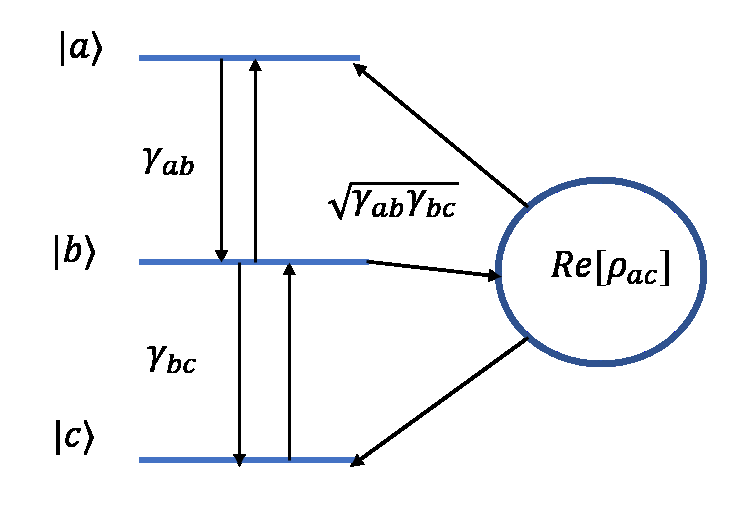
\includegraphics[width=0.9\columnwidth]{atom_fig3.eps}
\caption{(a) The steady state population distribution for different $\mu_{ab}$ and$\mu_{bc}$. The squeezing parameter $r=1$. (b) The steady state population distribution for non-ideal squeezed vacuum which is characterized by the ratio of $M$ and $\sqrt{N(N+1)}$.  The squeezing parameter $r=1$, and $\gamma_{ab}=\frac{1}{4}\gamma_{bc}$.}
\label{2}
\end{figure}
%\begin{equation}
%\label{eq4}
%\begin{split}
%\frac{d\rho^{S}}{dt}=&\sum_{i\ne j}\frac{\gamma}{2}[-\rho(\cosh rS_{i}^{\dagger}+\sinh rS_{j})(\cosh rS_{i}+\sinh rS_{j}^{\dagger})\\
%&-(\cosh rS_{i}^{\dagger}+\sinh rS_{j})(\cosh rS_{i}+\sinh rS_{j}^{\dagger})\rho\\
%&+2(\cosh rS_{i}+\sinh rS_{j}^{\dagger})\rho(\cosh rS_{i}^{\dagger}+\sinh rS_{j})]
%\end{split}
%\end{equation}

\begin{figure}
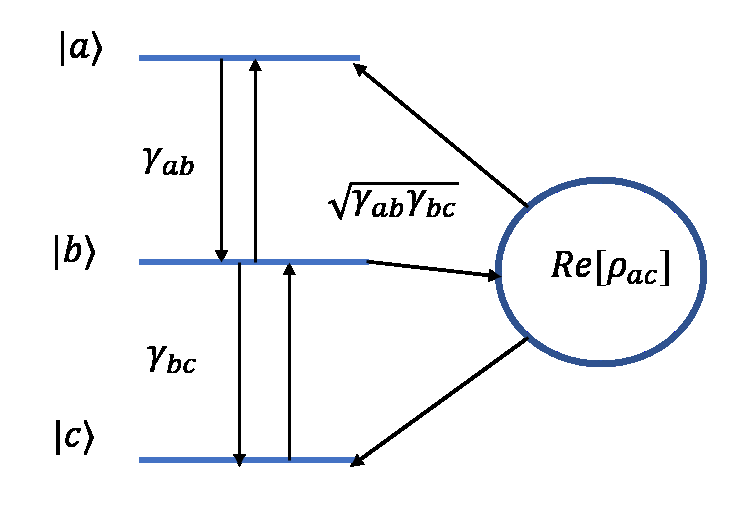
\includegraphics[width=0.8\columnwidth]{atom_fig3.eps}
\caption{ The allowed population flow in the squeezed vacuum.}
\label{2c}
\end{figure}

\section{steady state of multiple atoms}

In the last section, we demonstrate that arbitrary population inversion can occur for a single $\Xi$-type atom driven by the squeezed vacuum reservoir. However, with Eq.\eqref{eq2}, this result can not be generalized to the multi-atom case since $\gamma'_{ijij}=\sqrt{\gamma_{j}\gamma_{j}}\cos[2k_{0z}r_{i}]$. The squeezing term in Eq.\eqref{eq1} vanishes for atoms located around $r_i=\frac{\pi}{4k_{0z}}+\frac{n\pi}{2k_{0z}}$. Thus, for a group of randomly located atoms, if we want to achieve steady state population inversion in the squeezed vacuum, we need to modify our scheme. Here we consider the following correlation functions:
\begin{equation}
\label{eq0b}
\begin{split}
& \left\langle a_{\vec{k},s}^{\dagger}a_{\vec{k}',s'}\right\rangle =\sinh^{2}r\delta_{\vec{k}'\vec{k}}\delta_{ss'} \\
& \left\langle a_{\vec{k},s}a_{\vec{k}',s'}^{\dagger}\right\rangle =\cosh^{2}r\delta_{\vec{k}'\vec{k}}\delta_{ss'}\\
& \left\langle a_{\vec{k},s}^{\dagger}a_{\vec{k}',s'}^{\dagger}\right\rangle =-e^{-i\theta}\cosh(r)\sinh(r)\delta_{\vec{k}',-(2\vec{k}_{0}-\vec{k})}\delta_{ss'}\\
&\left\langle a_{\vec{k},s}a_{\vec{k}',s'}\right\rangle =-e^{i\theta}\cosh(r)\sinh(r)\delta_{\vec{k}',-(2\vec{k}_{0}-\vec{k})}\delta_{ss'}
\end{split}
\end{equation}
which indicates that photons are entangled with those from the opposite direction, then the coefficients in the the master equation Eq.\eqref{eq1} becomes 
\begin{equation}
\label{eq2b}
\begin{split}
& \gamma_{ijkl}=\sqrt{\gamma_{i}\gamma_{k}}\cos(k_{0z}r_{jl}) \\
& \Lambda_{ijkl}=\frac{\sqrt{\gamma_{i}\gamma_{k}}}{2}\sin(k_{0z}r_{jl})\\
& \gamma'_{ijkl}=\sqrt{\gamma_{i}\gamma_{k}}\cos(k_{0z}r_{jl})
\end{split}
\end{equation}
which is the traditionally studied master equation for atoms in squeezed reservoir \cite{tanas2004stationary}. The detailed derivation of the coefficients shown in Eq. (9) is given in Appendix B with the phase of the squeezing source included. Based on the master equation in Eq. (4) with coefficients given by Eq. (9), we can show that a single atom can reach population inversion anywhere in the waveguide, as discussed in the Sec. III. When there are multiple atoms in the waveguide where the dipole-dipole interaction should be considered, our calculation shows that the population inversion can still occur for all the atoms. In fact, the final state is just the direct product of the steady state of independent atoms, and this will be proved with the mathematical induction. Firstly, we need to apply the rotating wave approximation on Eq.\eqref{eq1}: 
\begin{widetext}
\begin{equation}
\label{eq5}
\begin{split}
\frac{d\rho^{S}}{dt}=&-i\underset{i,k,j}{\sum}\Lambda_{ijkl}[S_{i,j}^{+}S_{k.j}^{-},\rho^{S}]-\frac{1}{2}\underset{i,j,k}{\sum}\gamma{}_{ijkl}(1+N)(\rho^{S}S_{i,j}^{+}S_{k,j}^{-}+S_{i,j}^{+}S_{k,j}^{-}\rho^{S}-2S_{k,j}^{-}\rho^{S}S_{i,j}^{+}) \\
& -\frac{1}{2}\underset{i,j,k}{\sum}\gamma{}_{ijkl}N(\rho^{S}S_{i,j}^{-}S_{k,j}^{+}+S_{i,j}^{-}S_{k,j}^{+}\rho^{S}-2S_{k,j}^{+}\rho^{S}S_{i,j}^{-})\\
& -\frac{1}{2}\sum_{\alpha=\pm}\underset{i,k,j\ne l}{\sum}\gamma'_{ijkl}M(\rho^{S}S_{i,j}^{\alpha}S_{k,l}^{\alpha}+S_{i,j}^{\alpha}S_{k,l}^{\alpha}\rho^{S}-2S_{k,l}^{\alpha}\rho^{S}S_{i,j}^{\alpha})
\end{split}
\end{equation}
\end{widetext}

Assume that the steady state of N-atom system is $\rho^{S}=\rho_{1}\rho_{2}...\rho_{N}$ where $\rho_{i}=(A|a_{i}\rangle+C|c_{i}\rangle)(A\langle a_{i}|+C\langle c_{i}|)$ and $A=\frac{sh\sqrt{\gamma_{2}}}{\sqrt{ch^{2}\gamma_{1}+sh^{2}\gamma_{2}}}, C=-\frac{ch\sqrt{\gamma_{1}}}{\sqrt{ch^{2}\gamma_{1}+sh^{2}\gamma_{2}}}$. Then for $(N+1)$-atom case, the extra terms induced by the $(N+1)th$ atom on the right hand side of Eq.\eqref{eq5} are composed of three parts: $i=k=N+1$ terms, $i=N+1, k=1,2,\cdots,N$ terms, and $i=1,2,\cdots,N, k=N+1$ terms. The $i=k=N+1$ terms are the exact terms for the the $(N+1)th$ atom as a single independent atom, so the neat result of this term is 0. The terms with $i=N+1, k=1,2,\cdots, N$ are 
\begin{widetext}
\begin{equation}
\label{eq6}
\begin{split}
&-i\underset{j,k}{\sum}\Lambda_{N+1,j,k,j}[S_{N+1,j}^{+}S_{k.j}^{-},\rho^{S}] 
-\frac{1}{2}\underset{j,k}{\sum}\gamma{}_{N+1,j,k,j}(ch^{2})(\rho^{S}S_{N+1,j}^{+}S_{k,j}^{-}+S_{N+1,j}^{+}S_{k,j}^{-}\rho^{S}-2S_{k,j}^{-}\rho^{S}S_{N+1,j}^{+})\\
&-\frac{1}{2}\underset{j,k}{\sum}\gamma{}_{N+1,j,k,j}sh^{2}(\rho^{S}S_{N+1,j}^{-}S_{k,j}^{+}+S_{N+1,j}^{-}S_{k,j}^{+}\rho^{S}-2S_{k,j}^{+}\rho^{S}S_{N+1,j}^{-}) \\
&-\frac{1}{2}\sum_{\alpha=\pm}\underset{i,k,j\ne l}{\sum}\gamma'_{N+1,j,k,j}chsh(\rho^{S}S_{N+1,j}^{\alpha}S_{k,l}^{\alpha}+S_{N+1,j}^{\alpha}S_{k,l}^{\alpha}\rho^{S}-2S_{k,l}^{\alpha}\rho^{S}S_{N+1,j}^{\alpha})
\end{split}
\end{equation}
\end{widetext}
For the energy shift term (the first term) in expression \eqref{eq6}, we have 
\begin{equation}
\label{eq7}
\begin{split}
&S_{N+1,j}^{+}S_{k.j}^{-}\rho^{S}=\rho_{1}...(S_{k.j}^{-}\rho_{k})...\rho_{N}(S_{N+1,j}^{+}\rho_{N+1})=0\\
&\rho^{S}S_{N+1,j}^{+}S_{k.l}^{-}=\rho_{1}...(\rho_{k}S_{k.l}^{-})...\rho_{N}(\rho_{N+1}S_{N+1,j}^{+})=0
\end{split}
\end{equation}
For the thermal terms (the second and third terms) in expression \eqref{eq6}, we have:
\begin{equation}
\label{eq8}
\begin{split}
\rho^{S}S_{N+1,j}^{+}S_{k,j}^{-}=&S_{N+1,j}^{+}S_{k,j}^{-}\rho^{S}=0\\
\rho^{S}S_{N+1,j}^{-}S_{k,j}^{+}=&S_{N+1,j}^{-}S_{k,j}^{+}\rho^{S}=0\\
S_{k,j}^{-}\rho^{S}S_{N+1,j}^{+}=&\rho_{1}...(S_{k.j}^{-}\rho_{k})...\rho_{N}(\rho_{N+1}S_{N+1,j}^{+})\\
=&\rho_{1}...(S_{k.1}^{-}\rho_{k})...\rho_{N}(\rho_{N+1}S_{N+1,1}^{+})\\
=&\rho_{1}...(A|b_{k}\rangle)(A\langle a_{k}|+C\langle c_{k}|)..\rho_{N}\\
&\times(A|a_{N+1}\rangle+C|c_{N+1}\rangle)(A\langle b_{N+1}|)\\
S_{k,j}^{+}\rho^{S}S_{N+1,j}^{-}=&\rho_{1}...(S_{k.j}^{+}\rho_{k})...\rho_{N}(\rho_{N+1}S_{N+1,j}^{-})\\
=&\rho_{1}...(S_{k.2}^{+}\rho_{k})...\rho_{N}(\rho_{N+1}S_{N+1,2}^{-})\\
=&\rho_{1}...(C|b_{k}\rangle)(A\langle a_{k}|+C\langle c_{k}|)...\rho_{N}\\
&\times (A|a_{N+1}\rangle+C|c_{N+1}\rangle)(C\langle b_{N+1}|)
\end{split}
\end{equation}

For the squeezed vacuum terms(the forth term), we have:
\begin{equation}
\label{eq9}
\begin{split}
\rho^{S}S_{N+1,j}^{\alpha}S_{k,l}^{\alpha}&=S_{N+1,j}^{\alpha}S_{k,l}^{\alpha}\rho^{S}=0,\\
S_{k,1}^{+}\rho^{S}S_{N+1,2}^{+}&=\rho_{1}...(S_{k,1}^{+}\rho_{k})...\rho_{N}(\rho_{N+1}S_{N+1,2}^{+})=0,\\
S_{k,2}^{+}\rho^{S}S_{N+1,1}^{+}&=\rho_{1}...(S_{k,2}^{+}\rho_{k})...\rho_{N}(\rho_{N+1}S_{N+1,1}^{+})\\
&=\rho_{1}...(C|b_{k}\rangle)(A\langle a_{k}|+C\langle c_{k}|)...\rho_{N}\\
&\times(A|a_{N+1}\rangle+C|c_{N+1}\rangle)(A\langle b_{N+1}|),\\
S_{k,1}^{-}\rho^{S}S_{N+1,2}^{-}&=\rho_{1}...(S_{k,1}^{-}\rho_{k})...\rho_{N}(\rho_{N+1}S_{N+1,2}^{-})\\
&=\rho_{1}...(A|b_{k}\rangle)(A\langle a_{k}|+C\langle c_{k}|)...\rho_{N}\\
&\times(A|a_{N+1}\rangle+C|c_{N+1}\rangle)(C\langle b_{N+1}|),\\
S_{k,2}^{-}\rho^{S}S_{N+1,1}^{-}&=\rho_{1}...(S_{k,2}^{-}\rho_{k})...\rho_{N}(\rho_{N+1}S_{N+1,1}^{-})=0.\\
\end{split}
\end{equation}


\begin{figure*}
\includegraphics[width=0.66\columnwidth]{fig4a.eps}
\includegraphics[width=0.66\columnwidth]{fig4b.eps}
\includegraphics[width=0.66\columnwidth]{fig4c.eps}
\caption{(a)Fidelity evolution with different atomic separations. The atomic separations of $\lambda_0$, $0.1\lambda_0$, $0.2\lambda_0$ are plotted. Squeezing parameter $r=1$, decay rate $\frac{\gamma_1}{\gamma_2}=\frac{1}{4}$ and time unit $\tau=1/\sqrt{\gamma_{ab}\gamma_{bc}}$ is the geometric mean of the transition $|a\rangle\rightarrow|b\rangle$ and $|b\rangle\rightarrow|c\rangle$'s spontaneous emission rates in ordinary vacuum. (b) Fidelity evolution with different squeezing parameters. Decay rate $\frac{\gamma_1}{\gamma_2}=\frac{1}{4}$, and atomic separation $r_{12}=\lambda_0$. (c) Fidelity evolution with different decay rates. Squeezing parameter $r=1$, and atomic separation $r_{12}=\lambda_0$. }
\label{3}
\end{figure*}


Plugging Eq.\eqref{eq7}-\eqref{eq9} into expression \eqref{eq6}, we have
\begin{widetext}
\begin{equation}
\label{eq10}
\begin{split}
&\underset{k}{\sum}\gamma{}_{N+1,1,k,1}(ch^{2})S_{k,1}^{-}\rho^{S}S_{N+1,1}^{+}+\underset{j,k}{\sum}\gamma{}_{N+1,2,k,2}sh^{2}S_{k,2}^{+}\rho^{S}S_{N+1,2}^{-}
+\sum_{\alpha=\pm}\underset{i,k,j\ne l}{\sum}\gamma'_{N+1,j,k,l}chshS_{k,l}^{\alpha}\rho^{S}S_{N+1,j}^{\alpha}\\
=&\underset{k}{\sum}\gamma{}_{N+1,1,k,1}(ch^{2})\rho_{1}...(A|b_{k}\rangle)(A\langle a_{k}|+C\langle c_{k}|)..\rho_{N}(A|a_{N+1}\rangle+C|c_{N+1}\rangle)(A\langle b_{N+1}|)\\
&+\underset{k}{\sum}\gamma{}_{N+1,2,k,2}sh^{2}\rho_{1}...(C|b_{k}\rangle)(A\langle a_{k}|+C\langle c_{k}|)...\rho_{N}(A|a_{N+1}\rangle+C|c_{N+1}\rangle)(C\langle b_{N+1}|)\\
&+\underset{k}{\sum}\gamma'_{N+1,j,k,l}chsh[\rho_{1}...(C|b_{k}\rangle)(A\langle a_{k}|+C\langle c_{k}|)...\rho_{N}(A|a_{N+1}\rangle+C|c_{N+1}\rangle)(A\langle b_{N+1}|)\\
&+\rho_{1}...(A|b_{k}\rangle)(A\langle a_{k}|+C\langle c_{k}|)...\rho_{N}(A|a_{N+1}\rangle+C|c_{N+1}\rangle)(C\langle b_{N+1}|)]\\
=&\underset{k}{\sum}(\gamma{}_{N+1,1,k,1}ch^{2}A^{2}+\gamma{}_{N+1,2,k,2}sh^{2}C^{2}+2\gamma'_{N+1,j,k,l}chshCA)\\
&\times\rho_{1}...(|b_{k}\rangle)(A\langle a_{k}|+C\langle c_{k}|)..\rho_{N}(A|a_{N+1}\rangle+C|c_{N+1}\rangle)(\langle b_{N+1}|).
\end{split}
\end{equation}
\end{widetext}
Since $ch^{2}A^{2}\gamma{}_{N+1,1,k,1}+sh^{2}C^{2}\gamma{}_{N+1,2,k,2}+2chshCA\gamma'_{N+1,j,k,l}=0$, the extra terms induced by $i=N+1, k=1\sim N$ are 0. The same goes for $i=1\sim N, k=N+1$. Thus, the direct product of the steady state of single atom is also the steady state of the multiple atoms. It is interesting that the dipole-dipole interaction between the atoms doesn't have effects on the final steady state. Therefore, just like the single atom case, for multiple atoms, as long as their dipole directions are properly set, a population inversion of almost $100\%$ can be achieved for each atom. 

We also numerically show that steady state of multiple atoms is indeed the direct product of steady state of single atom. Since the cost for numerical simulation increases exponentially as the atom number increases, we only show the fidelity of two-atom state with respect to theoretical steady product state as a function of time in Fig.~\ref{3}, where the system is initially in the ground state. We can see that the system finally evolves into $\ensuremath{(\frac{sh\sqrt{\gamma_{2}}}{\sqrt{ch^{2}\gamma_{1}+sh^{2}\gamma_{2}}}|a_{1}\rangle-\frac{ch\sqrt{\gamma_{1}}}{\sqrt{ch^{2}\gamma_{1}+sh^{2}\gamma_{2}}}|c_{1}\rangle})(\frac{sh\sqrt{\gamma_{2}}}{\sqrt{ch^{2}\gamma_{1}+sh^{2}\gamma_{2}}}|a_{2}\rangle-\frac{ch\sqrt{\gamma_{1}}}{\sqrt{ch^{2}\gamma_{1}+sh^{2}\gamma_{2}}}|c_{2}\rangle)$ regardless of the atomic separation, squeezing parameter, and the ratio of decay rate $\gamma_{ab}/\gamma_{bc}$. In Fig. ~\ref{3}(b), it takes less time to evolve into the steady state for a smaller squeezing parameter. Fig. ~\ref{3}(c) shows that while smaller $\gamma_{ab}$ results in higher population inversion, it takes much longer for the system to evolve into the steady state.


 
\section{SUMMARY}
We study the $\Xi$-type atoms coupled to a broadband squeezed vacuum reservoir in a quasi-one-dimensional waveguide, with the overall transition frequency $\omega_{ac}=2\omega_0$. We show that a single atom will evolve into a steady state which is a superposition of the second excited state and the ground state. If the decay rate from the second excited state to the first excited state is much smaller than that from the first excited state to the ground state, the population can be almost $100\%$ trapped in the second excited state. What's more, we prove that the above result can be generalized to an arbitrary number of atoms interacting with each other via dipole-dipole interaction,and the system's final steady state is a direct product of that in the single-atom case. We also argue that the difference in decay rates of two transitions can be effectively achieved by polarizing the incident squeezed vacuum beam in the proper direction. 


\begin{widetext}
\appendix
\section{DERIVATION OF EQ.(4) }
Here we will show how to derive the master equation Eq. \eqref{eq1}. The interaction Hamiltonian is:
\begin{equation}
\label{eqa0}\tag{A1}
V(t)=-i\hbar \sum_{\vec{k}s}[D(t)a_{\vec{k}s}(t)-D^{+}(t)a^{\dagger}_{\vec{k}s}(t)],
\end{equation}
where
\begin{equation}
\label{eqa1}\tag{A2}
\begin{gathered}
D(t)=\underset{l,i}{\sum}[\vec{\mu}_{l,i}\cdot\vec{u}_{\vec{k},s}(r_{l,i})S_{l,i}^{\dagger}(t)+\vec{\mu}_{l,i}^{*}\cdot\vec{u}_{\vec{k},s}(r_{l,i})S_{l,i}^{-}(t)]
 \end{gathered}
\end{equation}
The reduced master equation of atoms in the reservoir is:
\begin{equation}
\label{eqa2}\tag{A3}
\begin{split}
\frac{d\rho^{S}}{dt}=&-\frac{1}{\hbar^{2}}\int_{0}^{t}d\tau Tr_{F}\{[V(t),[V(t-\tau),\rho^{S}(t-\tau)\rho^{F}\}\\
=&-\frac{1}{\hbar^{2}}\int_{0}^{t}d\tau Tr_{F}\{V(t)V(t-\tau)\rho^{S}(t-\tau)\rho^{F}+\rho^{S}(t-\tau)\rho^{F}V(t-\tau)V(t)\\
&-V(t)\rho^{S}(t-\tau)\rho^{F}V(t-\tau)-V(t-\tau)\rho^{S}(t-\tau)\rho^{F}V(t)\}
\end{split}
\end{equation} 
Here we just show how to deal with the first term in Eq.\eqref{eqa2}, the remaining terms can be calculated in the same way. For the first term, we have
\begin{equation}
\label{eqa3}\tag{A4}
\begin{split}
&-\frac{1}{\hbar^{2}}\int_{0}^{t}d\tau Tr_{F}\{V(t)V(t-\tau)\rho^{S}(t-\tau)\rho^{F}\}\\
=&\int_{0}^{t}d\tau\underset{\vec{k}s,\vec{k}'s'}{\sum}\{D(t)D(t-\tau)Tr_{F}[\rho^{F}a_{ks}(t)a_{k's'}(t-\tau)]-D(t)D^{+}(t-\tau)Tr_{F}[\rho^{F}a_{ks}(t)a^{\dagger}_{k's'}(t-\tau)]\\
&-D^{+}(t)D(t-\tau)Tr_{F}[\rho^{F}a^{\dagger}_{ks}(t)a_{k's'}(t-\tau)]+D^{+}(t)D^{+}(t-\tau)Tr_{F}[\rho^{F}a^{\dagger}_{ks}(t)a^{\dagger}_{k's'}(t-\tau)]\}\rho^{S}(t-\tau)\}.
\end{split}
\end{equation}
Under the rotating wave approximation(RWA), we have
\begin{equation}
\label{eqa4}\tag{A5}
\begin{split}
&-\frac{1}{\hbar^{2}}\int_{0}^{t}d\tau Tr_{F}\{V(t)V(t-\tau)\rho^{S}(t-\tau)\rho^{F}\}\\
=&\sum_{ijlm}\underset{\vec{k}s,\vec{k'}s'}{\sum}\int_{0}^{t}d\tau\{\vec{\mu}{}_{l,i}\cdot\vec{u}_{\vec{k}s}(r_{l,i})S_{l,i}^{+}e^{i\omega_{i}t}\vec{\mu}_{m,j}\cdot\vec{u}_{\vec{k}'s'}(r_{m,j})S_{m,j}^{+}e^{i\omega_{j}(t-\tau)}e^{-i(\omega_{\vec{k}s}+\omega_{\vec{k}'s'})t+i\omega_{\vec{k}'s'}\tau}[-\sinh(r)\cosh(r)\delta_{\vec{k}',2\vec{k}_{0}-\vec{k}}\delta_{ss'}]\\
&-\vec{\mu}_{l,i}\cdot\vec{u}_{\vec{k}s}(r_{l,i})S_{l,i}^{+}e^{i\omega_{i}t}\vec{\mu}_{m,j}^{*}\cdot\vec{u}_{\vec{k}'s'}^{*}(r_{m,j})S_{m,j}^{-}e^{-i\omega_{j}(t-\tau)}e^{-i\omega_{\vec{k}'s'}\tau}\cosh^{2}r\delta_{\vec{k}\vec{k}'}\delta_{ss'}\\
&-\vec{\mu}_{l,i}^{*}\cdot\vec{u}_{\vec{k}s}(r_{l,i})S_{l,i}^{-}e^{-i\omega_{i}t}\vec{\mu}_{m,j}\cdot\vec{u}_{\vec{k}'s'}^{*}(r_{m,j})S_{m,j}^{+}e^{i\omega_{j}(t-\tau)}e^{-i\omega_{\vec{k}'s'}\tau}\cosh^{2}r\delta_{\vec{k}\vec{k}'}\delta_{ss'}\\
&-\vec{\mu}_{l,i}^{*}\cdot\vec{u}_{\vec{k}s}^{*}(r_{l,i})S_{l,i}^{-}e^{-i\omega_{i}t}\vec{\mu}_{m,j}\cdot\vec{u}_{\vec{k}'s'}(r_{m,j})S_{m,j}^{+}e^{i\omega_{j}(t-\tau)}e^{i\omega_{\vec{k}'s'}\tau}\sinh^{2}r\delta_{\vec{k}\vec{k}'}\delta_{ss'}\\
&-\vec{\mu}_{l,i}\cdot\vec{u}_{\vec{k}s}^{*}(r_{l,i})S_{l,i}^{+}e^{i\omega_{i}t}\vec{\mu}_{m,j}^{*}\cdot\vec{u}_{\vec{k}'s'}(r_{m,j})S_{m,j}^{-}e^{-i\omega_{j}(t-\tau)}e^{i\omega_{\vec{k}'s'}\tau}\sinh^{2}r\delta_{\vec{k}\vec{k}'}\delta_{ss'}\\
&+\vec{\mu}_{l,i}^{*}\cdot\vec{u}_{\vec{k}s}^{*}(r_{l,i})S_{l,i}^{-}e^{-i\omega_{i}t}\vec{\mu}_{m,j}^{*}\cdot\vec{u}_{\vec{k}'s'}^{*}(r_{m,j})S_{m,j}^{-}e^{-i\omega_{j}(t-\tau)}e^{i(\omega_{\vec{k}s}+\omega_{\vec{k}'s'})t-i\omega_{\vec{k}'s'}\tau}[-\sinh(r)\cosh(r)\delta_{\vec{k}',2\vec{k}_{0}-\vec{k}}\delta_{ss'}]\}\rho^{S}(t-\tau)
\end{split}
\end{equation}
where $l,m$ are used for labeling different atoms, and $i,j$ are used for transitions within an atom. Here we just calculate the first and second term to show how to get the master equation Eq.\eqref{eq1}. Since all atoms are identical, $\omega_{l,i}=\omega_{i}$, $|\vec\mu_{l,i}|=|\vec\mu_i|$, and $r_{l,i}=r_{l}$ can be used to simplify Eq.\eqref{eqa4}. For simplicity, we define $\mu_j$ to be the projection of $\vec{mu_j}$ on the $x$ axis. For the second term(thermal term), we have
\begin{equation}
\label{eqc2}\tag{A6}
\begin{split}
&-\underset{k_{z}}{\sum}\int_{0}^{t}d\tau\vec{\mu}_{l,i}\cdot\vec{u}_{\vec{k}s}(r_{l})S_{l,i}^{+}e^{i\omega_{i}t}\vec{\mu}_{m,j}^{*}\cdot\vec{u}_{\vec{k}'s'}^{*}(r_{m})S_{m,j}^{-}e^{-i\omega_{j}(t-\tau)}e^{-i\omega_{\vec{k}'s'}\tau}\cosh^{2}r\rho^{S}(t-\tau)\delta_{\vec{k}\vec{k}'}\delta_{ss'}\\
=&-\frac{L}{2\pi}e^{i(\omega_{i}-\omega_{j})t}\int_{-\infty}^{\infty}dk_{z}\int_{0}^{t}d\tau e^{i\omega_{j}\tau}e^{-i\omega_{k_{z}}\tau}\frac{\omega_{k}\mu_{i}\mu_{j}}{\epsilon_{0}LS\hbar}e^{ik_{z}(r_{l}-r_{m})}\cosh^{2}rS_{l,i}^{+}S_{m,j}^{-}\rho^{S}(t-\tau)\\
\approx&-\frac{L}{2\pi}e^{i(\omega_{i}-\omega_{j})t}\int_{0}^{\infty}dk_{z}\int_{0}^{t}d\tau e^{i\omega_{j}\tau}e^{-i[\omega_{j}+c^{2}k_{jz}(k_{z}-k_{jz})/\omega_{j}]\tau}\frac{\omega_{k}\mu_{i}\mu_{j}}{\epsilon_{0}LS\hbar}[e^{ik_{z}(r_{l}-r_{m})}+e^{-ik_{z}(r_{l}-r_{m})}]\cosh^{2}rS_{l,i}^{+}S_{m,j}^{-}\rho^{S}(t-\tau)\\
\approx&-\frac{L}{2\pi}e^{i(\omega_{i}-\omega_{j})t}\int_{-k_{0z}}^{\infty}d\delta k_{z}\int_{0}^{t}d\tau e^{-i\tau c^{2}k_{jz}\delta k_{z}/\omega_{j}}\frac{\omega_{k}\mu_{i}\mu_{j}}{\epsilon_{0}LS\hbar}[e^{i(k_{jz}+\delta k_{z})(r_{l}-r_{m})}+e^{-i(k_{jz}+\delta k_{z})(r_{l}-r_{m})}]\cosh^{2}rS_{l,i}^{+}S_{m,j}^{-}\rho^{S}(t-\tau)\\
\approx&-\frac{L}{2\pi}e^{i(\omega_{i}-\omega_{j})t}\int_{-\infty}^{\infty}d\delta k_{z}\int_{0}^{t}d\tau e^{-i(c^{2}k_{jz}\delta k_{z}/\omega_{j})\tau}\frac{\omega_{k}\mu_{i}\mu_{j}}{\epsilon_{0}LS\hbar}[e^{i(k_{jz}+\delta k_{z})(r_{l}-r_{m})}+e^{-i(k_{jz}+\delta k_{z})(r_{l}-r_{m})}]\cosh^{2}rS_{l,i}^{+}S_{m,j}^{-}\rho^{S}(t-\tau)\\
\approx&-\frac{L}{2\pi}e^{i(\omega_{i}-\omega_{j})t}\int_{0}^{t}d\tau\frac{\omega_{j}\mu_{i}\mu_{j}}{\epsilon_{0}LS\hbar}2\pi[e^{ik_{jz}(r_{l}-r_{m})}\delta((r_{l}-r_{m})-\frac{c^{2}k_{jz}}{\omega_{0}}\tau)+e^{-ik_{jz}(r_{l}-r_{m})}\delta((r_{l}-r_{m})+\frac{c^{2}k_{jz}}{\omega_{0}}\tau)]\cosh^{2}rS_{l,i}^{+}S_{m,j}^{-}\rho^{S}(t-\tau)\\
\approx&-\frac{L}{2\pi}e^{ik_{jz}r_{lm}}\frac{\omega_{j}\mu_{i}\mu_{j}}{\epsilon_{0}LS\hbar}2\pi\frac{\omega_{j}}{c^{2}k_{0z}}\cosh^{2}rS_{l,i}^{+}S_{m,j}^{-}\rho^{S}(t)e^{i(\omega_{i}-\omega_{j})t}\\
\approx&-[\frac{\sqrt{\gamma_{i}\gamma_{j}}}{2}\cos(k_{0z}r_{lm})+i\frac{\sqrt{\gamma_{i}\gamma_{j}}}{2}sin(k_{0z}r_{lm})]\cosh^{2}rS_{l,i}^{+}S_{m,j}^{-}\rho^{S}(t)e^{i(\omega_{i}-\omega_{j})t}\\
\end{split}
\end{equation}
where emitter separation $r_{lm}=|r_{l}-r_{m}|$, collective decay rate $\gamma_{i}=2\mu_{i}^{2}\omega_{i}^{2}/\hbar\epsilon_{0}Sc^{2}k_{iz}$, and collective energy shift $\Lambda_{ij}=\sqrt{\gamma_{i}\gamma_{j}}\sin(k_{0z}r_{ij})/2$.
In the third line we expand $\omega_{k}=c\sqrt{(\frac{\pi}{a})^{2}+(k_{z})^{2}}$ around $k_{z}=k_{0z}$ since resonant modes provide dominant contributions. In the fifth line we extend the integration $\int_{-k_{jz}}^{\infty}dk_{z}\rightarrow\int_{-\infty}^{\infty}dk_{z}$ because the main contribution comes from the components around $\delta k_{z}=0$. In the next line, Weisskopf-Wigner approximation is used. Thus, we have obtained $\gamma_{ij}$ and $\Lambda_{ij}$ as is shown in Eq.\eqref{eq2}. 

Next we need to calculate the first term (squeezing term) in Eq.\eqref{eqa4}:
\begin{equation}
\label{eqb8}\tag{A7}
\begin{split}
& e^{i(\omega_{i}+\omega_{j}-2\omega_{0})t}\underset{k_{z}}{\sum}\int_{0}^{t}d\tau\{\vec{\mu}{}_{l,i}\cdot\vec{u}_{2\vec{k}_{0}-\vec{k}}(r_{l})S_{l,i}^{+}\vec{\mu}_{m,j}\cdot\vec{u}_{\vec{k}}(r_{m})S_{m,j}^{+}e^{i(\omega_{\vec{k}}-\omega_{j})\tau}[-\sinh(r)\cosh(r)]\rho^{S}(t-\tau)\\
=&-\frac{L}{2\pi}e^{i(\omega_{i}+\omega_{j}-2\omega_{0})t}\int_{0}^{2k_{0z}}dk_{z}\int_{0}^{t}d\tau e^{i(\omega_{k_{z}}-\omega_{j})\tau}e^{i(2k_{jz}-k_{z})(r_{l}-o_{1})}e^{ik_{z}(r_{m}-o_{1})}\frac{\sqrt{\omega_{k_{z}}\omega_{2k_{0z}-k_{z}}}\mu_{i}\mu_{j}}{\epsilon_{0}LS\hbar}\sinh(r)\cosh(r)S_{l,i}^{+}S_{m,j}^{+}\rho^{S}(t-\tau)\\ 
&-\frac{L}{2\pi}e^{i(\omega_{i}+\omega_{j}-2\omega_{0})t}\int_{-2k_{0z}}^{0}dk_{z}\int_{0}^{t}d\tau e^{i(\omega_{k_{z}}-\omega_{j})\tau}e^{i(-2k_{jz}-k_{z})(r_{l}-o_{2})}e^{ik_{z}(r_{m}-o_{2})}\frac{\sqrt{\omega_{k_{z}}\omega_{-2k_{0z}-k_{z}}}\mu_{i}\mu_{j}}{\epsilon_{0}LS\hbar}\sinh(r)\cosh(r)S_{l,i}^{+}S_{m,j}^{+}\rho^{S}(t-\tau)
\end{split}
\end{equation}
Putting aside the overall factor $e^{i(\omega_i+\omega_j-2\omega_0)t}$, for $r_l=r_j$, Eq.\eqref{eqb8} reduces to 
\begin{equation}
\label{eqb9}\tag{A8}
\begin{split}
&\underset{k_{z}}{\sum}\int_{0}^{t}d\tau\{\vec{\mu}{}_{l,i}\cdot\vec{u}_{2\vec{k}_{0}-\vec{k}}(r_{l})S_{l,i}^{+}\vec{\mu}_{l,j}\cdot\vec{u}_{\vec{k}}(r_{l})S_{l,j}^{+}e^{i(\omega_{\vec{k}}-\omega_{j})\tau}[-\sinh(r)\cosh(r)]\rho^{S}(t-\tau)\\
=&-\frac{L}{2\pi}\int_{0}^{2k_{0z}}dk_{z}\int_{0}^{t}d\tau e^{i\frac{c^{2}k_{jz}}{_{\omega_{j}}}(k_{z}-k_{jz})\tau}e^{i2k_{0z}(r_{l}-o_{1})}\frac{\sqrt{\omega_{k_{z}}\omega_{2k_{0z}-k_{z}}}\mu_{i}\mu_{j}}{\epsilon_{0}LS\hbar}\sinh(r)\cosh(r)S_{l,i}^{+}S_{l,j}^{+}\rho^{S}(t-\tau)\\
&-\frac{L}{2\pi}\int_{-2k_{0z}}^{0}dk_{z}\int_{0}^{t}d\tau e^{i\frac{c^{2}k_{jz}}{_{\omega_{j}}}(k_{z}-k_{jz})\tau}e^{-i2k_{0z}(r_{l}-o_{2})}\frac{\sqrt{\omega_{k_{z}}\omega_{-2k_{0z}-k_{z}}}\mu_{i}\mu_{j}}{\epsilon_{0}LS\hbar}\sinh(r)\cosh(r)S_{l,i}^{+}S_{l,j}^{+}\rho^{S}(t-\tau)\\
=&-\frac{L}{2\pi}[e^{i2k_{0z}(r_{l}-o_{1})}+e^{-i2k_{0z}(r_{l}-o_{2})}]\frac{\sqrt{\omega_{i}\omega_{j}}\mu_{i}\mu_{j}}{\epsilon_{0}LS\hbar}\int_{0}^{t}d\tau2\pi\delta(\frac{c^{2}k_{jz}}{\omega_{j}}\tau)\sinh(r)\cosh(r)S_{l,i}^{+}S_{l,j}^{+}\rho^{S}(t-\tau)\\
=&-e^{i2k_{jz}R}\frac{\omega_{0}^{2}\mu_{i}\mu_{j}}{\epsilon_{0}\hbar Sc^{2}k_{0z}}\cos(2k_{0z}r_{l})\sinh(r)\cosh(r)S_{l,i}^{+}S_{l,j}^{+}\rho^{S}(t)\\
=&-e^{i2k_{0z}R}\frac{\sqrt{\gamma_{i}\gamma_{j}}}{2}\cos(2k_{0z}r_{l})\sinh(r)\cosh(r)S_{l,i}^{+}S_{l,j}^{+}\rho^{S}(t)
\end{split}
\end{equation}
where we have used the fact that the origin of coordinate system is at equal distant from two sources(i.e., $o_2=-o_1=R$) in the second last line. Incorporating index $l$ into $i$, we have $\gamma'_{ij}=\sqrt{\gamma_{i}\gamma_{j}}\cos(2k_{0z}r_{i})$. For $r_i\neq r_j$, Eq. \eqref{eqb8} reduces to
\begin{equation}
\label{eqb10}\tag{A9}
\begin{split}
&\underset{k_{z}}{\sum}\int_{0}^{t}d\tau\{\vec{\mu}{}_{l,i}\cdot\vec{u}_{2\vec{k}_{0}-\vec{k}}(r_{l})S_{l,i}^{+}\vec{\mu}_{m,j}\cdot\vec{u}_{\vec{k}}(r_{m})S_{m,j}^{+}e^{i(\omega_{\vec{k}}-\omega_{j})\tau}[-\sinh(r)\cosh(r)]\rho^{S}(t-\tau)\\
=&-\frac{L}{2\pi}\int_{0}^{2k_{0z}}dk_{z}\int_{0}^{t}d\tau e^{i\frac{c^{2}k_{jz}}{_{\omega_{j}}}(k_{z}-k_{jz})\tau}e^{i2k_{0z}(r_{c}-o_{1})}e^{-i(k_{z}-k_{0z})(r_{l}-r_{m})}\frac{\sqrt{\omega_{k_{z}}\omega_{2k_{0z}-k_{z}}}\mu_{i}\mu_{j}}{\epsilon_{0}LS\hbar}\sinh(r)\cosh(r)S_{l,i}^{+}S_{m,j}^{+}\rho^{S}(t-\tau) \\
& -\frac{L}{2\pi}\int_{-2k_{0z}}^{0}dk_{z}\int_{0}^{t}d\tau e^{i\frac{c^{2}k_{jz}}{_{\omega_{j}}}(-k_{z}-k_{jz})\tau}e^{-i2k_{0z}(r_{c}-o_{2})}e^{-i(k_{z}+k_{0z})(r_{l}-r_{m})}\frac{\sqrt{\omega_{k_{z}}\omega_{-2k_{0z}-k_{z}}}\mu_{i}\mu_{j}}{\epsilon_{0}LS\hbar}\sinh(r)\cosh(r)S_{l,i}^{+}S_{m,j}^{+}\rho^{S}(t-\tau)\\
=&-\frac{L}{2\pi}e^{i2k_{0z}(r_{c}-o_{1})}\frac{\sqrt{\omega_{i}\omega_{j}}\mu_{i}\mu_{j}}{\epsilon_{0}LS\hbar}\int_{-\infty}^{\infty}dk_{z}\int_{0}^{t}d\tau e^{i\frac{c^{2}k_{jz}}{_{\omega_{j}}}(k_{z}-k_{jz})\tau}e^{-i(k_{z}-k_{0z})(r_{l}-r_{m})}\sinh(r)\cosh(r)S_{l,i}^{+}S_{m,j}^{+}\rho^{S}(t-\tau)\\
&-\frac{L}{2\pi}e^{-i2k_{0z}(r_{c}-o_{2})}\frac{\sqrt{\omega_{i}\omega_{j}}\mu_{i}\mu_{j}}{\epsilon_{0}LS\hbar}\int_{-\infty}^{\infty}dk_{z}\int_{0}^{t}d\tau e^{i\frac{c^{2}k_{jz}}{_{\omega_{j}}}(k_{z}-k_{jz})\tau}e^{i(k_{z}-k_{0z})(r_{l}-r_{m})}\sinh(r)\cosh(r)S_{l,i}^{+}S_{m,j}^{+}\rho^{S}(t-\tau) \\
\approx&-\frac{L}{2\pi}e^{i2k_{0z}R}\frac{\omega_{0}^{2}\mu_{i}\mu_{j}}{\epsilon_{0}LS\hbar}\int_{0}^{t}d\tau2\pi[e^{i2k_{0z}r_{c}}\delta(r_{l}-r_{m}-\frac{c^{2}k_{0z}}{_{\omega_{0}}}\tau)+e^{-i2k_{0z}r_{c}}\delta(r_{l}-r_{m}+\frac{c^{2}k_{0z}}{_{\omega_{0}}}\tau)]\sinh(r)\cosh(r)S_{l,i}^{+}S_{m,j}^{+}\rho^{S}(t-\tau) \\
\approx&-e^{i2k_{0z}R}\frac{\omega_{0}^{2}\mu_{i}\mu_{j}}{\epsilon_{0}\hbar Sc^{2}k_{0z}}e^{i2k_{0z}r_{c}sgn(r_{l}-r_{m})}S_{l,i}^{+}S_{m,j}^{+}\rho^{S}(t)\rightarrow-\frac{\sqrt{\gamma_{i}\gamma_{j}}}{2}e^{i2k_{0z}R}\cos(k_{0z}(r_{l}+r_{m}))S_{l,i}^{+}S_{m,j}^{+}\rho^{S}(t)\\
\end{split}
\end{equation}
where $sgn(r_{l}-r_{m})$ is the sign function. The last arrow is because we need to sum over $i,j$, so the imaginary part of $e^{i2k_{0z}r_{c}sgn(i-j)}$ vanishes, so the neat result is that $\gamma'_{ijkl}=e^{i2k_{0z}R}\sqrt{\gamma_{j}\gamma_{l}}\cos(k_{0z}(r_{i}+r_{k}))$. As for $S_{i}^{+}\rho^{S}(t)S_{j}^{+}$ terms, the combination of the last two terms in Eq.\eqref{eqa2} will make the imaginary part of $e^{i2k_{0z}r_{c}sgn(r_{l}-r_{m})}$ vanish. Thus, we have $\gamma'_{ijkl}$ in Eq.\eqref{eq2}. 

\section{DERIVATION OF coefficients EQ.(9) }
Here we will show how to derive the master equation with coefficients Eq.\eqref{eq2b}. The mode function of the squeezed vacuum is given by
\begin{equation}
  \label{eq2b}
  \begin{gathered}
\vec{u}_{\vec{k}s}(\vec{r}_{i})=\sqrt{\frac{\omega_{\vec{k}s}}{2\epsilon_{0}\hbar V}}\vec{e}_{ks}e^{i\vec{k}\cdot(\vec{r}_{i}-\vec{o}_{\vec{k}s})}
 \end{gathered}
\end{equation}
where $\vec{o}_{\vec{k}s} $ is a phenomenological parameter which includes the effects of the initial phase and the position of the squeezing source\cite{You2018}. The correlation functions for the squeezed vacuum are\cite{scully1999quantum}:
\begin{equation}
\label{eq0a}
\begin{split}
& \left\langle a_{\vec{k},s}^{\dagger}a_{\vec{k}',s'}\right\rangle =\sinh^{2}r\delta_{\vec{k}'\vec{k}}\delta_{ss'} \\
& \left\langle a_{\vec{k},s}a_{\vec{k}',s'}^{\dagger}\right\rangle =\cosh^{2}r\delta_{\vec{k}'\vec{k}}\delta_{ss'}\\
& \left\langle a_{\vec{k},s}^{\dagger}a_{\vec{k}',s'}^{\dagger}\right\rangle =-e^{-i\theta}\cosh(r)\sinh(r)\delta_{\vec{k}',2\vec{k}_{0}-\vec{k}}\delta_{ss'}\\
&\left\langle a_{\vec{k},s}a_{\vec{k}',s'}\right\rangle =-e^{i\theta}\cosh(r)\sinh(r)\delta_{\vec{k}',2\vec{k}_{0}-\vec{k}}\delta_{ss'}
\end{split}
\end{equation}
For simplicity, we can set the squeezing parameter $\theta=0$, and all atoms to align along the same direction.

 Since the only difference is the squeezing terms $\left\langle a_{\vec{k},s}^{\dagger}a_{\vec{k}',s'}^{\dagger}\right\rangle$, $\left\langle a_{\vec{k},s}a_{\vec{k}',s'}\right\rangle $, we will just start from Eq. \eqref{eqb8}. Apart from the factor $e^{i(\omega_i+\omega_j-2\omega_0)t}$, When $r_i\ne r_j$, Eq. \eqref{eqb8} becomes:

\begin{equation}
\label{eqb1}\tag{B1}
\begin{split}
&\underset{k_{z}}{\sum}\int_{0}^{t}d\tau\{\vec{\mu}{}_{l,i}\cdot\vec{u}_{-2\vec{k}_{0}+\vec{k}}(r_{l})S_{l,i}^{+}\vec{\mu}_{m,j}\cdot\vec{u}_{\vec{k}}(r_{m})S_{m,j}^{+}e^{i(\omega_{\vec{k}}-\omega_{0})\tau}[-\sinh(r)\cosh(r)]\rho^{S}(t-\tau)\\
\approx&-\frac{L}{2\pi}\int_{0}^{2k_{0}}dk\int_{0}^{t}d\tau e^{i\frac{c^{2}k_{0}}{_{\omega_{0}}}(k-k_{0})\tau}e^{-i(2k_{0}-k)(r_{l}-o_{2})+ik(r_{m}-o_{1})}\frac{\sqrt{\omega_{k_{z}}\omega_{2k_{0z}-k_{z}}}\mu_{i}\mu_{j}}{\epsilon_{0}LS\hbar}\sinh(r)\cosh(r)S_{l,i}^{+}S_{m,j}^{+}\rho^{S}(t-\tau)\\
&-\frac{L}{2\pi}\int_{-2k_{0}}^{0}dk\int_{0}^{t}d\tau e^{i\frac{c^{2}k_{0}}{_{\omega_{0}}}(-k-k_{0})\tau}e^{i(2k_{0}+k)(r_{l}-o_{2})+ik(r_{m}-o_{1})}\frac{\sqrt{\omega_{k_{z}}\omega_{-2k_{0z}-k_{z}}}\mu_{i}\mu_{j}}{\epsilon_{0}LS\hbar}\sinh(r)\cosh(r)S_{l,i}^{+}S_{m,j}^{+}\rho^{S}(t-\tau)\\
=&-\frac{L}{2\pi}\int_{0}^{2k_{0}}dk\int_{0}^{t}d\tau e^{i\frac{c^{2}k_{0}}{_{\omega_{0}}}(-k_{0})\tau}e^{-i(2k_{0})(r_{l}-o_{2})}e^{ik(\frac{c^{2}k_{0}}{_{\omega_{0}}}\tau+r_{l}-o_{1}+r_{m}-o_{2})}\frac{\sqrt{\omega_{k_{z}}\omega_{2k_{0z}-k_{z}}}\mu_{i}\mu_{j}}{\epsilon_{0}LS\hbar}\sinh(r)\cosh(r)S_{l,i}^{+}S_{m,j}^{+}\rho^{S}(t-\tau)\\
&-\frac{L}{2\pi}\int_{0}^{2k_{0}}dk\int_{0}^{t}d\tau e^{i\frac{c^{2}k_{0}}{_{\omega_{0}}}(-k_{0})\tau}e^{i(2k_{0})(r_{l}-o_{2})}e^{ik(\frac{c^{2}k_{0}}{_{\omega_{0}}}\tau-r_{l}+o_{1}-r_{m}+o_{2})}\frac{\sqrt{\omega_{k_{z}}\omega_{-2k_{0z}-k_{z}}}\mu_{i}\mu_{j}}{\epsilon_{0}LS\hbar}\sinh(r)\cosh(r)S_{l,i}^{+}S_{m,j}^{+}\rho^{S}(t-\tau)\\
\approx&-\frac{L}{2\pi}\int_{0}^{t}d\tau e^{i\frac{c^{2}k_{0}}{_{\omega_{0}}}(-k_{0})\tau}e^{-i(2k_{0})(r_{l})}e^{2ik_{0}o_{2}}2\pi\delta(\frac{c^{2}k_{0}}{_{\omega_{0}}}\tau+2r_{c}-o_{1}-o_{2})\frac{\sqrt{\omega_{i}\omega_{j}}\mu_{i}\mu_{j}}{\epsilon_{0}LS\hbar}\sinh(r)\cosh(r)S_{l,i}^{+}S_{m,j}^{+}\rho^{S}(t-\tau)\\
&-\frac{L}{2\pi}\int_{0}^{t}d\tau e^{i\frac{c^{2}k_{0}}{_{\omega_{0}}}(-k_{0})\tau}e^{i(2k_{0})(r_{l})}e^{-2ik_{0}o_{2}}2\pi\delta(\frac{c^{2}k_{0}}{_{\omega_{0}}}\tau-2r_{c}+o_{1}+o_{2})\frac{\sqrt{\omega_{i}\omega_{j}}\mu_{i}\mu_{j}}{\epsilon_{0}LS\hbar}\sinh(r)\cosh(r)S_{l,i}^{+}S_{m,j}^{+}\rho^{S}(t-\tau)\\
\approx&-\frac{L}{2\pi}e^{i(-k_{0})|2r_{c}-o_{1}-o_{2}|}e^{sgn(r_{c}-o_{1}-o_{2})i(2k_{0})(r_{l})}e^{-2ik_{0}o_{2}}2\pi\frac{\omega_{0}^{2}\mu_{i}\mu_{j}}{\epsilon_{0}LS\hbar c^{2}k_{0z}}\sinh(r)\cosh(r)S_{l,i}^{+}S_{m,j}^{+}\rho^{S}(t)\\
=&-\frac{L}{2\pi}e^{sgn(2r_{c}-o_{1}-o_{2})ik_{0}(r_{l}-r_{m})}e^{ik_{0}(o_{1}-o_{2})}2\pi\frac{\omega_{0}^{2}\mu_{i}\mu_{j}}{\epsilon_{0}LS\hbar c^{2}k_{0z}}\sinh(r)\cosh(r)S_{l,i}^{+}S_{m,j}^{+}\rho^{S}(t)
\end{split}
\end{equation}
Since we need to sum over $l,m,i,j$, the imaginary part of $e^{sgn(2r_{c}-o_{1}-o_{2})ik_{0}(r_{l}-r_{m})}$ gets canceled, which yields $\gamma'_{ijkl}=\sqrt{\gamma_{i}\gamma_{k}}\cos[k_{0z}(r_{jl})]$. The above calculation is also valid when $r_i=r_j$.


\end{widetext}

\bibliography{ref}
\begin{thebibliography}{99}
\end{thebibliography}
%
%\begin{thebibliography}{28}
%\expandafter\ifx\csname natexlab\endcsname\relax\def\natexlab#1{#1}\fi
%\expandafter\ifx\csname bibnamefont\endcsname\relax
%  \def\bibnamefont#1{#1}\fi
%\expandafter\ifx\csname bibfnamefont\endcsname\relax
%  \def\bibfnamefont#1{#1}\fi
%\expandafter\ifx\csname citenamefont\endcsname\relax
%  \def\citenamefont#1{#1}\fi
%\expandafter\ifx\csname url\endcsname\relax
%  \def\url#1{\texttt{#1}}\fi
%\expandafter\ifx\csname urlprefix\endcsname\relax\def\urlprefix{URL }\fi
%\providecommand{\bibinfo}[2]{#2}
%\providecommand{\eprint}[2][]{\url{#2}}
%
%\bibitem[{\citenamefont{Svelto and Hanna}(1998)}]{svelto1998principles}
%\bibinfo{author}{\bibfnamefont{O.}~\bibnamefont{Svelto}} \bibnamefont{and}
%  \bibinfo{author}{\bibfnamefont{D.~C.} \bibnamefont{Hanna}},
%  \emph{\bibinfo{title}{Principles of lasers}}, vol.~\bibinfo{volume}{4}
%  (\bibinfo{publisher}{Springer}, \bibinfo{year}{1998}).
%
%\bibitem[{\citenamefont{Purcell}(1946)}]{purcell1946purcell}
%\bibinfo{author}{\bibfnamefont{E.}~\bibnamefont{Purcell}},
%  \bibinfo{journal}{Phys. Rev.} \textbf{\bibinfo{volume}{69}},
%  \bibinfo{pages}{681} (\bibinfo{year}{1946}).
%
%\bibitem[{\citenamefont{Gardiner}(1986)}]{gardiner1986cw}
%\bibinfo{author}{\bibfnamefont{C.}~\bibnamefont{Gardiner}},
%  \bibinfo{journal}{Phys. Rev. Lett.} \textbf{\bibinfo{volume}{56}},
%  \bibinfo{pages}{1917} (\bibinfo{year}{1986}).
%
%\bibitem[{\citenamefont{Collett}(1984)}]{collett1984mj}
%\bibinfo{author}{\bibfnamefont{M.}~\bibnamefont{Collett}},
%  \bibinfo{journal}{Phys. Rev. A} \textbf{\bibinfo{volume}{30}},
%  \bibinfo{pages}{1386} (\bibinfo{year}{1984}).
%
%\bibitem[{\citenamefont{Gea-Banacloche
%  et~al.}(1988)\citenamefont{Gea-Banacloche, Scully, and
%  Zubairy}}]{gea1988vacuum}
%\bibinfo{author}{\bibfnamefont{J.}~\bibnamefont{Gea-Banacloche}},
%  \bibinfo{author}{\bibfnamefont{M.}~\bibnamefont{Scully}}, \bibnamefont{and}
%  \bibinfo{author}{\bibfnamefont{M.}~\bibnamefont{Zubairy}},
%  \bibinfo{journal}{Physica Scripta} \textbf{\bibinfo{volume}{1988}},
%  \bibinfo{pages}{81} (\bibinfo{year}{1988}).
%
%\bibitem[{\citenamefont{Palma}(1989)}]{palma1989gm}
%\bibinfo{author}{\bibfnamefont{G.}~\bibnamefont{Palma}}, \bibinfo{journal}{Opt.
%  Commun.} \textbf{\bibinfo{volume}{73}}, \bibinfo{pages}{131}
%  (\bibinfo{year}{1989}).
%
%\bibitem[{\citenamefont{Agarwal and Puri}(1990)}]{agarwal1990cooperative}
%\bibinfo{author}{\bibfnamefont{G.}~\bibnamefont{Agarwal}} \bibnamefont{and}
%  \bibinfo{author}{\bibfnamefont{R.}~\bibnamefont{Puri}},
%  \bibinfo{journal}{Physical Review A} \textbf{\bibinfo{volume}{41}},
%  \bibinfo{pages}{3782} (\bibinfo{year}{1990}).
%
%\bibitem[{\citenamefont{Ficek}(1990)}]{ficek1990spontaneous}
%\bibinfo{author}{\bibfnamefont{Z.}~\bibnamefont{Ficek}},
%  \bibinfo{journal}{Physical Review A} \textbf{\bibinfo{volume}{42}},
%  \bibinfo{pages}{611} (\bibinfo{year}{1990}).
%
%\bibitem[{\citenamefont{Ficek}(1991)}]{ficek1991z}
%\bibinfo{author}{\bibfnamefont{Z.}~\bibnamefont{Ficek}},
%  \bibinfo{journal}{Phys. Rev. A} \textbf{\bibinfo{volume}{44}},
%  \bibinfo{pages}{7759} (\bibinfo{year}{1991}).
%
%\bibitem[{\citenamefont{Goldstein}(1996)}]{goldstein1996ev}
%\bibinfo{author}{\bibfnamefont{E.}~\bibnamefont{Goldstein}},
%  \bibinfo{journal}{Phys. Rev. A} \textbf{\bibinfo{volume}{53}},
%  \bibinfo{pages}{3573} (\bibinfo{year}{1996}).
%
%\bibitem[{\citenamefont{Carmichael et~al.}(1987)\citenamefont{Carmichael, Lane,
%  and Walls}}]{carmichael1987}
%\bibinfo{author}{\bibfnamefont{H.}~\bibnamefont{Carmichael}},
%  \bibinfo{author}{\bibfnamefont{A.}~\bibnamefont{Lane}}, \bibnamefont{and}
%  \bibinfo{author}{\bibfnamefont{D.}~\bibnamefont{Walls}},
%  \bibinfo{journal}{Physical review letters} \textbf{\bibinfo{volume}{58}},
%  \bibinfo{pages}{2539} (\bibinfo{year}{1987}).
%
%\bibitem[{\citenamefont{Toyli et~al.}(2016)\citenamefont{Toyli, Eddins, Boutin,
%  Puri, Hover, Bolkhovsky, Oliver, Blais, and Siddiqi}}]{toyli2016resonance}
%\bibinfo{author}{\bibfnamefont{D.}~\bibnamefont{Toyli}},
%  \bibinfo{author}{\bibfnamefont{A.}~\bibnamefont{Eddins}},
%  \bibinfo{author}{\bibfnamefont{S.}~\bibnamefont{Boutin}},
%  \bibinfo{author}{\bibfnamefont{S.}~\bibnamefont{Puri}},
%  \bibinfo{author}{\bibfnamefont{D.}~\bibnamefont{Hover}},
%  \bibinfo{author}{\bibfnamefont{V.}~\bibnamefont{Bolkhovsky}},
%  \bibinfo{author}{\bibfnamefont{W.}~\bibnamefont{Oliver}},
%  \bibinfo{author}{\bibfnamefont{A.}~\bibnamefont{Blais}}, \bibnamefont{and}
%  \bibinfo{author}{\bibfnamefont{I.}~\bibnamefont{Siddiqi}},
%  \bibinfo{journal}{Physical Review X} \textbf{\bibinfo{volume}{6}},
%  \bibinfo{pages}{031004} (\bibinfo{year}{2016}).
%
%
%
%\bibitem[{\citenamefont{Tana{\'s} and Ficek}(2004)}]{tanas2004stationary}
%\bibinfo{author}{\bibfnamefont{R.}~\bibnamefont{Tana{\'s}}} \bibnamefont{and}
%  \bibinfo{author}{\bibfnamefont{Z.}~\bibnamefont{Ficek}},
%  \bibinfo{journal}{Journal of Optics B: Quantum and Semiclassical Optics}
%  \textbf{\bibinfo{volume}{6}}, \bibinfo{pages}{S610} (\bibinfo{year}{2004}).
%
%\bibitem[{\citenamefont{Li et~al.}(2006)\citenamefont{Li, Peng, and
%  Yin}}]{li2006preparing}
%\bibinfo{author}{\bibfnamefont{F.-L.} \bibnamefont{Li}},
%  \bibinfo{author}{\bibfnamefont{P.}~\bibnamefont{Peng}}, \bibnamefont{and}
%  \bibinfo{author}{\bibfnamefont{Z.-Q.} \bibnamefont{Yin}},
%  \bibinfo{journal}{Journal of Modern Optics} \textbf{\bibinfo{volume}{53}},
%  \bibinfo{pages}{2055} (\bibinfo{year}{2006}).
%
%\bibitem[{\citenamefont{You et~al.}(2018)\citenamefont{You, Liao, Li, and
%  Zubairy}}]{You2018}
%\bibinfo{author}{\bibfnamefont{J.}~\bibnamefont{You}},
%  \bibinfo{author}{\bibfnamefont{Z.}~\bibnamefont{Liao}},
%  \bibinfo{author}{\bibfnamefont{S.-W.} \bibnamefont{Li}}, \bibnamefont{and}
%  \bibinfo{author}{\bibfnamefont{M.~S.} \bibnamefont{Zubairy}},
%  \bibinfo{journal}{Physical Review A} \textbf{\bibinfo{volume}{97}},
%  \bibinfo{pages}{023810} (\bibinfo{year}{2018}).
%
%\bibitem[{\citenamefont{Ficek and Drummond}(1991)}]{ficek1991three}
%\bibinfo{author}{\bibfnamefont{Z.}~\bibnamefont{Ficek}} \bibnamefont{and}
%  \bibinfo{author}{\bibfnamefont{P.}~\bibnamefont{Drummond}},
%  \bibinfo{journal}{Physical Review A} \textbf{\bibinfo{volume}{43}},
%  \bibinfo{pages}{6247} (\bibinfo{year}{1991}).
%
%\bibitem[{\citenamefont{Ficek and Drummond}(1993)}]{ficek1993two}
%\bibinfo{author}{\bibfnamefont{Z.}~\bibnamefont{Ficek}} \bibnamefont{and}
%  \bibinfo{author}{\bibfnamefont{P.}~\bibnamefont{Drummond}},
%  \bibinfo{journal}{EPL (Europhysics Letters)} \textbf{\bibinfo{volume}{24}},
%  \bibinfo{pages}{455} (\bibinfo{year}{1993}).
%
%\bibitem[{\citenamefont{Shen and Fan}(2005)}]{shen2005coherent}
%\bibinfo{author}{\bibfnamefont{J.-T.} \bibnamefont{Shen}} \bibnamefont{and}
%  \bibinfo{author}{\bibfnamefont{S.}~\bibnamefont{Fan}},
%  \bibinfo{journal}{Physical review letters} \textbf{\bibinfo{volume}{95}},
%  \bibinfo{pages}{213001} (\bibinfo{year}{2005}).
%
%\bibitem[{\citenamefont{Shen and Fan}(2007)}]{shen2007strongly}
%\bibinfo{author}{\bibfnamefont{J.-T.} \bibnamefont{Shen}} \bibnamefont{and}
%  \bibinfo{author}{\bibfnamefont{S.}~\bibnamefont{Fan}},
%  \bibinfo{journal}{Physical review letters} \textbf{\bibinfo{volume}{98}},
%  \bibinfo{pages}{153003} (\bibinfo{year}{2007}).
%
%\bibitem[{\citenamefont{Yudson and Reineker}(2008)}]{yudson2008multiphoton}
%\bibinfo{author}{\bibfnamefont{V.}~\bibnamefont{Yudson}} \bibnamefont{and}
%  \bibinfo{author}{\bibfnamefont{P.}~\bibnamefont{Reineker}},
%  \bibinfo{journal}{Physical Review A} \textbf{\bibinfo{volume}{78}},
%  \bibinfo{pages}{052713} (\bibinfo{year}{2008}).
%
%\bibitem[{\citenamefont{Liao et~al.}(2015)\citenamefont{Liao, Zeng, Zhu, and
%  Zubairy}}]{liao2015single}
%\bibinfo{author}{\bibfnamefont{Z.}~\bibnamefont{Liao}},
%  \bibinfo{author}{\bibfnamefont{X.}~\bibnamefont{Zeng}},
%  \bibinfo{author}{\bibfnamefont{S.-Y.} \bibnamefont{Zhu}}, \bibnamefont{and}
%  \bibinfo{author}{\bibfnamefont{M.~S.} \bibnamefont{Zubairy}},
%  \bibinfo{journal}{Phys. Rev. A} \textbf{\bibinfo{volume}{92}},
%  \bibinfo{pages}{023806} (\bibinfo{year}{2015}).
%
%\bibitem[{\citenamefont{Liao et~al.}(2016)\citenamefont{Liao, Nha, and
%  Zubairy}}]{liao2016dynamical}
%\bibinfo{author}{\bibfnamefont{Z.}~\bibnamefont{Liao}},
%  \bibinfo{author}{\bibfnamefont{H.}~\bibnamefont{Nha}}, \bibnamefont{and}
%  \bibinfo{author}{\bibfnamefont{M.~S.} \bibnamefont{Zubairy}},
%  \bibinfo{journal}{Phys. Rev. A} \textbf{\bibinfo{volume}{94}},
%  \bibinfo{pages}{053842} (\bibinfo{year}{2016}).
%  
%  \bibitem[{\citenamefont{Liao et~al.}(2016)\citenamefont{Liao, Zeng, Nha, and
%  Zubairy}}]{liao2016review}
%\bibinfo{author}{\bibfnamefont{Z.}~\bibnamefont{Liao}},
%\bibinfo{author}{\bibfnamefont{X.}~\bibnamefont{Zeng}},
%  \bibinfo{author}{\bibfnamefont{H.}~\bibnamefont{Nha}}, \bibnamefont{and}
%  \bibinfo{author}{\bibfnamefont{M.~S.} \bibnamefont{Zubairy}},
%  \bibinfo{journal}{Phys. Scr.} \textbf{\bibinfo{volume}{91}},
%  \bibinfo{pages}{063004} (\bibinfo{year}{2016}).
%  
%  \bibitem[{\citenamefont{Roy et~al.}(2017)\citenamefont{Roy, Wilson, and
%  Firstenberg}}]{roy2017review}
%\bibinfo{author}{\bibfnamefont{D.}~\bibnamefont{Roy}},
%\bibinfo{author}{\bibfnamefont{C.}~\bibnamefont{Wilson}}, \bibnamefont{and}
%  \bibinfo{author}{\bibfnamefont{O.} \bibnamefont{Firstenberg}},
%  \bibinfo{journal}{Rev. Mod. Phys.} \textbf{\bibinfo{volume}{89}},
%  \bibinfo{pages}{021001} (\bibinfo{year}{2017}).
%
%\bibitem[{\citenamefont{Turchette}(1998)}]{turchette1998qa}
%\bibinfo{author}{\bibfnamefont{Q.}~\bibnamefont{Turchette}},
%  \bibinfo{journal}{Phys. Rev. A} \textbf{\bibinfo{volume}{58}},
%  \bibinfo{pages}{4056} (\bibinfo{year}{1998}).
%
%\bibitem[{\citenamefont{Murch}(2013)}]{murch2013kw}
%\bibinfo{author}{\bibfnamefont{K.}~\bibnamefont{Murch}},
%  \bibinfo{journal}{Nature (London)} \textbf{\bibinfo{volume}{499}},
%  \bibinfo{pages}{62} (\bibinfo{year}{2013}).
%
%\bibitem[{\citenamefont{Bergeal et~al.}(2010)\citenamefont{Bergeal, Vijay,
%  Manucharyan, Siddiqi, Schoelkopf, Girvin, and Devoret}}]{bergeal2010analog}
%\bibinfo{author}{\bibfnamefont{N.}~\bibnamefont{Bergeal}},
%  \bibinfo{author}{\bibfnamefont{R.}~\bibnamefont{Vijay}},
%  \bibinfo{author}{\bibfnamefont{V.}~\bibnamefont{Manucharyan}},
%  \bibinfo{author}{\bibfnamefont{I.}~\bibnamefont{Siddiqi}},
%  \bibinfo{author}{\bibfnamefont{R.}~\bibnamefont{Schoelkopf}},
%  \bibinfo{author}{\bibfnamefont{S.}~\bibnamefont{Girvin}}, \bibnamefont{and}
%  \bibinfo{author}{\bibfnamefont{M.}~\bibnamefont{Devoret}},
%  \bibinfo{journal}{Nature Physics} \textbf{\bibinfo{volume}{6}},
%  \bibinfo{pages}{296} (\bibinfo{year}{2010}).
%
%\bibitem[{\citenamefont{Wang et~al.}(2018)\citenamefont{Wang, Shankar, Minev,
%  Campagne-Ibarcq, Narla, and Devoret}}]{wang2018cavity}
%\bibinfo{author}{\bibfnamefont{Z.}~\bibnamefont{Wang}},
%  \bibinfo{author}{\bibfnamefont{S.}~\bibnamefont{Shankar}},
%  \bibinfo{author}{\bibfnamefont{Z.}~\bibnamefont{Minev}},
%  \bibinfo{author}{\bibfnamefont{P.}~\bibnamefont{Campagne-Ibarcq}},
%  \bibinfo{author}{\bibfnamefont{A.}~\bibnamefont{Narla}}, \bibnamefont{and}
%  \bibinfo{author}{\bibfnamefont{M.}~\bibnamefont{Devoret}},
%  \bibinfo{journal}{arXiv preprint arXiv:1807.04849}  (\bibinfo{year}{2018}).
%
%\bibitem[{\citenamefont{Qin et~al.}(2018)\citenamefont{Qin, Miranowicz, Li,
%  L{\"u}, You, and Nori}}]{qin2018exponentially}
%\bibinfo{author}{\bibfnamefont{W.}~\bibnamefont{Qin}},
%  \bibinfo{author}{\bibfnamefont{A.}~\bibnamefont{Miranowicz}},
%  \bibinfo{author}{\bibfnamefont{P.-B.} \bibnamefont{Li}},
%  \bibinfo{author}{\bibfnamefont{X.-Y.} \bibnamefont{L{\"u}}},
%  \bibinfo{author}{\bibfnamefont{J.-Q.} \bibnamefont{You}}, \bibnamefont{and}
%  \bibinfo{author}{\bibfnamefont{F.}~\bibnamefont{Nori}},
%  \bibinfo{journal}{Physical review letters} \textbf{\bibinfo{volume}{120}},
%  \bibinfo{pages}{093601} (\bibinfo{year}{2018}).
%
%\bibitem[{\citenamefont{Scully and Zubairy}(1999)}]{scully1999quantum}
%\bibinfo{author}{\bibfnamefont{M.~O.} \bibnamefont{Scully}} \bibnamefont{and}
%  \bibinfo{author}{\bibfnamefont{M.~S.} \bibnamefont{Zubairy}},
%  \emph{\bibinfo{title}{Quantum optics}} (\bibinfo{year}{1999}).
%
%\end{thebibliography}

\end{document}